% book example for classicthesis.sty
\documentclass[
  % Replace twoside with oneside if you are printing your thesis on a single side
  % of the paper, or for viewing on screen.
  oneside,
  %twoside,
  11pt, a4paper,
  footinclude=true,
  headinclude=true,
  cleardoublepage=empty
]{scrbook}

\setlength{\marginparwidth}{2cm}

\usepackage{indentfirst}
\usepackage{dissertation}
\usepackage{float}
%---
\usepackage[T1]{fontenc}
\usepackage{textcomp}
%---
\usepackage[titles]{tocloft}
%% Aesthetic spacing redefines that look nicer to me than the defaults.
\setlength{\cftbeforechapskip}{2ex}
\setlength{\cftbeforesecskip}{0.5ex}
%% Use Helvetica-Narrow Bold for Chapter entries
\renewcommand{\cftpartfont}{%
  \fontsize{12}{14}\usefont{OT1}{phv}{bc}{n}\selectfont
}
\renewcommand{\cftchapfont}{%
  \fontsize{11}{13}\usefont{OT1}{phv}{bc}{n}\selectfont
}
\renewcommand{\cftsecfont}{%
  \fontsize{10}{11}\usefont{OT1}{phv}{}{n}\selectfont
}
\renewcommand{\cftsubsecfont}{%
  \fontsize{9}{10}\usefont{OT1}{phv}{}{n}\selectfont
}
\renewcommand{\cftfigfont}{%
  \fontsize{9}{10}\usefont{OT1}{phv}{}{n}\selectfont
}
\renewcommand{\cfttabfont}{%
  \fontsize{9}{10}\usefont{OT1}{phv}{}{n}\selectfont
}
%---
%usepackage[scaled=.92]{helvet}
\usepackage[all]{xy}
\usepackage{circuitikz}

\titleclass{\subsubsubsection}{straight}[\subsection]


% Title

\titleA{Formalizing ROS2 security configuration with Alloy}

% Author

\author{Luís Mário Macedo Ribeiro}

% Supervisor(es)

\supervisor{Manuel Alcino Pereira da Cunha}

\cosupervisorA{André Filipe Faria dos Santos}

% Date

\date{\myear} % change to text if date is not today

%\makeglossaries %  either use this ...

\makeindex	% ... or this

\begin{document}\fontfamily{phv}\fontseries{mc}\selectfont

% Add acronym definitions

% Cover page ---------------------------------------------
%	\thispagestyle{empty}
	%!TEX root = dissertation.tex

\makeatletter

% UM_ENg Logo
\def\UMEng#1#2{\begin{tikzpicture}[
	% bars styling,
	logone/.style={rectangle,fill=white,rounded corners=0.08cm,minimum width=0.16cm,inner sep=0pt},
	bigone/.style={minimum height=0.74cm},
	smaone/.style={minimum height=0.48cm},
	engone/.style={minimum height=0.86cm},
	pos1/.style={xshift=1.3cm,yshift=1.3cm},
	pos2/.style={xshift=3.9cm,yshift=1.3cm}]
	
% Uminho logo
	\fill[fill=#1] (0,0) -- (2.6,0) -- (2.6,2.6) -- (0,2.6) -- cycle;
	\foreach \i in {1,...,3}{
		\node at (\i*120+30:0.45)[logone,bigone,pos1,rotate=\i*120-60]{};
		\node at (\i*120+90:0.60)[logone,smaone,pos1,rotate=\i*120]{};
	}

% EngUminho logo
	\fill[fill=#2] (2.6,0) -- (5.2,0) -- (5.2,2.6) -- (2.6,2.6) -- cycle;
	\foreach \i in {1,...,5}
		\node at (\i*72-90:0.74)[engone,logone,pos2,rotate=\i*72-90]{};
\end{tikzpicture}}

\def\yyy#1{\fontfamily{phv}\fontseries{mc}\selectfont {\ifnum\hide=1\relax\else#1\fi}}
\def\xxx#1{\fontfamily{phv}\fontseries{mc}\selectfont #1}
\def\zzz#1{\fontfamily{phv}\fontseries{mc}\fontseries{b}\selectfont #1}
\def\kkk#1{\fontfamily{phv}\fontseries{mc}\fontseries{b}\selectfont {\ifnum\hide=1\relax\else#1\fi}}

\long\def\coverEtc{
%Logo
~\vskip-4.1cm\rule{4cm}{0pt}\begin{tabular}{l}
\UMEng\umc{eng}
\\\zzz{Universidade do Minho}\rule{0pt}{1cm}
\\\xxx{}{Escola de Engenharia}
\\\xxx{Departamento de  Informática}
\\\rule{0pt}{4cm}
\\\xxx{{\Large\@author}}
\\\rule{0pt}{1em}
\\\zzz{\Large\@titleA}
\\\zzz{\Large\@titleB}
\\\zzz{\Large\@titleC}
\\\rule{0pt}{5cm}
\\\yyy{\large Master dissertation}
\\\yyy{\large Integrated Master’s in Informatics Engineering}
\\\rule{0pt}{6mm}
\\\yyy{\large Dissertation supervised by}
\\\kkk{\@supervisor}\rule{0pt}{4mm}
\\\kkk{\@cosupervisor}
\\\rule{0pt}{4.2cm}
\\\xxx{{\small\@date}}
\end{tabular}
}


\begin{frontcover}
\gdef\umc{um}\gdef\hide{1}
\thispagestyle{empty} \pagecolor{white} \textcolor{black} \coverEtc
\end{frontcover}

\begin{titlepage}
\gdef\umc{um}
\gdef\hide{0}
\thispagestyle{empty} \pagecolor{white}\textcolor{grey} \coverEtc
\end{titlepage}

\makeatother


%rm
	\cleardoublepage
%---------------------------------------------------------
	\pagenumbering{gobble}
	\setcounter{page}{0}
%---------------------------------------------------------
% Add acknowledgements

\chapter*{Copyright and Terms of Use for Third Party Work}

\noindent This dissertation reports on academic work that can be used by third parties as long as the internationally accepted standards and good practices are respected concerning copyright and related rights.
\vskip 1em
\noindent This work can thereafter be used under the terms established in the license below.
\vskip 1em
\noindent Readers needing authorization conditions not provided for in the indicated licensing should contact the author through the RepositóriUM of the University of Minho.

\section*{License granted to users of this work:}

\CCBY % or replace by one in***************** the list below, cf https://alunos.uminho.pt/PT/estudantes/Formataes/3_Despacho_RT-31_2019_Anexo%203-Informa%c3%a7%c3%a3o-Direitor%20de%20Autor.docx
%---------
%\CBYNCND
%\CCBYNCSA
%\CCBYNC
%\CCBYND
%\CCBYSA


%---------

\chapter*{Acknowledgements}
% Write your acknowledgements here. Do not forget to mention the projects and grants that you have benefited from while doing your research, if any. Ask your supervisor about the specific textual format to use. (Funding agencies are quite strict about this.)

	\cleardoublepage

%---------

\chapter*{Statement of Integrity}

\noindent I hereby declare having conducted this academic work with integrity.
\vskip 1em\noindent
I confirm that I have not used plagiarism or any form of undue use of information or falsification of results along the process leading to its elaboration.
\vskip 1em\noindent
I further declare that I have fully acknowledged the Code of Ethical Conduct of the University of Minho.

%---------

% Uncomment as wished

% Add abstracts (en,pt) -----------------------------------------------------------
\chapter*{Abstract}
	
	Industrial restructuring is becoming highly reliant on automation developments, as they bring more efficient and accurate processes with less associated cost. Consequently, robots are rapidly being deployed in a wide range of scenarios, especially where security is demanded. In such cases, it is critical to employ appropriate procedures to verify both the system's quality, as well as its security.

	Following the current growth of cyber-physical system, as well as their usage into various technology domains, the development of software applications is demanding due to the complexity behind the integration of needed services, beyond those provided by the operating system. Hereupon, software middleware is increasingly used, since it offers services that support application development and delivery.

	One of the most popular open-source software platforms for building robotic systems is the Robot Operating System (ROS) \cite{1} middleware, where highly configurable robots are usually built by composing third-party modules. A major factor behind its popularity and widespread adoption is its flexibility and interoperability. One drawback of this flexibility, however, lies in the increased security risks that ROS applications face. Alongisde security risks, the arising of performance and scalability issues related to the ROS middleware specification, compelled the development of ROS2.

	Robot Operating System 2 (ROS2), which continues to provide a simple, uniform message passing interface to allow components to communicate with each other, is implemented using the Data Distribution Service (DDS) \cite{3} communication protocol, where security guarantees are ensured by DDS-Security specification. Using DDS-Security, it is possible to configure ROS2 to run with security guarantees using the SROS2 toolset \cite{ros-dds-integration}. However, improper configuration can still lead security problems.
	
	This thesis proposes a technique, based on the software verification perspective, to automatically verify system-wide properties related to the security configuration of ROS2-based applications. The intended purpose is to model the ROS architecture, as well as the network communication behaviour, in Alloy \cite{alloy-6}, a formal specification language and analysis tool supported by a model-finder over which, system-wide properties are subsequently model-checked.

\paragraph{Keywords} Robotics, ROS, ROS2, DDS, SROS2, Security, Software Verification, Alloy
	\cleardoublepage

\chapter*{Resumo}

	A constante implementação da ideia de automização de processos tem motivado a reestruturação nos mais diversos setores industriais, com o obejtivo de aumentar a eficiência e precisão nos processos integrados, consequentemente, reduzindo os custos associados. Além disso, esta ideia impulsiona a integração robótica nos mais amplos domínios tecnológicos, especialmente em domínios onde a segurança é exigida. Nestes casos, é fundamental adotar técnicas apropriadas de forma a verificar tanto a qualidade do sistema, como a segurança do mesmo.

	Como resultado do atual crescimento de sistemas ciber-físicos, nomeadamente sistemas robóticos, bem como sua utilização em vários domínios tecnológicos, o desenvolvimento de aplicações é exigente devido à complexidade da integração dos serviços necessários, tipicamente não fornecidos pelo sistema operativo. De forma a acompanhar o aumento da complexidade destes sistemas, \textit{middlewares} têm sido adoptados, pois integram serviços que oferecem suporte ao desenvolvimento de aplicações robóticas.

	Uma das plataformas considerada como \textit{standard} no que toca ao desenvolvimento sistemas robóticos é o middleware Robot Operating System (ROS) \cite{1}, onde robôs altamente configuráveis são construídos atráves da composição modular de \textit{software} externo, oferencedo características como flexibilidade e interoperabilidade aos sistemas integrados. No entanto, a constante priorização na flexibilidade resulta num aumento de vulnerabilidades de segurança, pondo em causa a integridade das aplicações. Além da falta de segurança apresentada, existem também problemas de desempenho e escalabilidade relacionados com a especificação do \textit{middleware}. Assim, era necessário uma mudança na estruturação do ROS, resultando na criação do Robot Operating System 2 (ROS2).

	O Robot Operating System 2 (ROS2) implementa um protocolo de comunicação, de nome Data Distribution Service (DDS) \cite{3}, que para além de garantir serviços de comunicação, fornece diversas especificações, onde diversas implementações DDS usufruem de tais especificações. A especificação DDS-Security, que através de uma metodologia de \textit{plugins}, oferece diferentes métodos de adoção de segurança. Através do uso desta especificação, juntamente com o uso do SROS2 \textit{toolset} \cite{ros-dds-integration}, é possível configurar o ROS2 de forma a adotar estas medidas de segurança.

	Esta tese propõe uma técnica para a verificação automática de \textit{system-wide properties} em aplicações ROS. Esta técnica apresentada baseia-se na formalização estrutural de arquiteturas ROS em Alloy \cite{alloy-6}, com o obejtivo de modelar o comportamento associado à comunicação dentro do sistema, tendo em consideração configurações associadas às propriedades de segurança. 
	
	
\paragraph{Palavras-chave} Robótica, ROS, ROS2, DDS, SROS2, Segurança, Verificação de Software, Alloy


	\cleardoublepage

	\pagenumbering{roman}
	\setcounter{page}{3}
	%pagestyle{fancy}   % -------- removed
	%rm

	% Document
	\cleardoublepage
    \phantomsection
	\tableofcontents

	\cleardoublepage
	\listoffigures

	%\cleardoublepage
	%\listoftables

	%\cleardoublepage
	%\lstlistoflistings

	% Add list of acronyms
	\cleardoublepage
	\pagenumbering{arabic}
	\setcounter{page}{3}

\part{Introductory material}

\chapter{Introduction}\label{c:intro}

Robots have emerged into our world as they are used routinely to perform quests done traditionally by human beings. The decreasing cost of robots is one of the main reasons for their increased use.\cite{craig2005introduction} Economics aside, the usage of robots brings increased productivity, safety and more manufacturing production work back to developed countries.\cite{robots-importance} Robotics is already the key driver of competitiveness and flexibility in large scale manufacturing industries.\cite{robots-everyday-life} 

Robotics is significantly reliant on a variety of technologies, connected into the same robotic system. Due to the continuous growth of technology in these different domains, robots can be used in a wide range of applications.\cite{mohamed2008middleware}

Developing and writing software code for robot applications is demanding, where multiple aspects must be considered properly, as the complexity of robotics is continuously growing. Robots tend to be designed for a particular purpose, resulting in a wide variety of hardware combined, consequently making already written software code extremely difficult to understand and implement, so the complexity behind is demanding. Typically, code perception and reasoning are way to complex for any single programmer, when abstraction strategies are not taking into account. Even though, many robotics researchers have previously created frameworks to deal with these problems, simplifying complexity issues by providing rapid prototyping, they tend to not scale to feature a wide community of robotics programmers. ROS aims to solve this concern, by providing a modular package-based framework, designed to be built upon by robot software developers. Their software can then be utilized by a variety of platforms and applications.\cite{intro-ros}

The Robot Operating System was created by a collaborative open-source community to contribute in the advancement of robots.\cite{diluoffo2018robot} that enables locomotion, manipulation, navigation, and recognition tasks, complemented by software libraries and tools with the aim of helping build robot applications easily, without the need of building it from scratch. ROS was designed to be flexible, since working with robots requires experimentation, given the variety of different hardware and software. This flexibility enables the combination between existing components with new ones. 


\section{Problem Statement}\label{s:problem}

As reliance on robotic systems increases,  
% Robotic systems, so called \textbf{Cyber-physical} systems, besides concerning about its realiability as a trusted system, must prioritize 
concerns such as time efficiency and distribution are considered as priority. % Systems that rely on distribution, referred as a distributed system, supports the idea of no centralization of the systems components, by dispersing them across the systems network and handling communication by message-passing. 
System distribution relates to the productivity matters, making robotic systems more flexible, by allowing robot compoisiton into the same network. Systems that relie on time effiency meets real-time constraints, called deadlines, mainly concerns about safety, since robots can directly affect human lifes. However, robotic systems need to be responsive, to expect maximum productivity, especially when its being considered a distributed network that rely on different robotic components. 

Formerly, robots were designed to complete certain single tasks, so they tended to build as one unit. However, robots are now composed by components concerned by a shared distributed network, promoting the ideia of connecting different hardware and software modules that provide control over these components. The integrated robot's modules coop together to complete a shared purpose. Since these software modules can have distinguished specification, the integration between them raises interoperability and communication issues, so the complexity behind the robots application development must be addressed by a middle layer, the \textbf{middleware}. The main idea behind implementing a middleware into a distributed system, is to ease the development cost, while provide interoperability and communication facilitation.\cite{mohamed2008middleware} The requirement for a middleware layer that meets different robot's specfication is a novel approach to enable the creation of robot applications over robotic systems, while supporting features such as robustness and modularity. 

In real-time distributed systems, middleware for robotics development must meet stringent requirements.\cite{maruyama2016exploring} The former version of ROS, was previously considered as an open-source middleware, as they provided their own middleware implementation. However, performance and scalability issues arised due to its middleware specification.\cite{intro-ros} Additionally, real-time constraints such as fault-tolerance, deadlines, or process synchronization were not supported by ROS, making it unsuitable for safety-critical and real-time systems.\cite{kim2018security} 

Besides having no middleware support for distributed real-time systems, security features were also not featured by ROS, which started to be demanding for deployed systems. An increasing number of real-time applications, for instance robotic systems, requires security ensurance for protecting real-time sensive data, against unauthorized access.\cite{lin2009static} 
Previously, robotic systems were protected using a static environment, usually closed networks. The need for robotics evolution demanded a change of approach, where systems must be acessible and extendable from the public network, allowing flexibility within the network, at the cost of security.

This lead to the creation of Robot Operating System 2, which continues to provide a simple, uniform message passing interface to allow components to communicate with each other, now implemented using the Data Distribution Service (DDS)\cite{3} specification protocol as its middleware, leveraging for its messaging architecture. Issues concerning system integration and scalability are mitigated by DDS various implementations, due to the several transport configurations provided, making it suitable for real-time distributed systems. DDS also provides a security specifcation, called DDS-Security, used by multiple implementations, and ROS2 makes use of them to provide features to the deployed robotic systems.\cite{8442103}


\section{Objectives and Contributions}

The first goal of this thesis rests in introducing concepts around the Robot Operating System, contextualizing the evolution behind its framework towards achieving security, where the former version of ROS lacked due to the focus on flexibility. Since ROS2 has been developed over the DDS framework, as its communication middleware, DDS must be properly understood before considering the security aspects. To do so, simple examples will first be studied and introduced, in order to provide ROS-based context to the reader. The domain of autonomous systems, where security is of extreme relevance, namely the Autoware\cite{8443742} ROS2 platform for self-driving vehicles will also be introduced. To understand SROS2 we intend to configure and run a realistic case study related to Autoware with security guarantees. 

The DDS Security standard functionality is evaluated, as well as how security is integrated into ROS2. Since security issues, concerning public networks, are recent to the robotics domain, ROS2 security network design should be analysed structurally.

Security configuration related to SROS2 toolset will be provided in this chapter, supported by an example that accounts multiple security features, those being authentication, encryption and, most importantly, access control, applying restriction constraints to the network and its participants, that by default are not controlled.

The second goal is to extend a previously proposed\cite{9341085} formalization of ROS applications in Alloy/Electrum\cite{alloy-DJ, lwspecification} to also take into consideration the security configuration defined with SROS2. Using this extension, we intend to explore the viability of verifying simple information-flow security properties. For instance, to ensure that no commands to the vehicle motor can be sent via the infotainment system.

The final goal is to automate the extraction of such formal Alloy models from the configuration files of a ROS2 application, in order to obtain a prototype tool that can be used by roboticists to easily detect security configuration issues.

\section{Document Structure}

The current pre-dissertation document is divided into 4 different chapters, namely: Robot Operating System (\ref{c:ros}), Alloy Specification Framework (\ref{c:alloy}), Current work (\ref{c:currWork}) and Conclusion and Future work (\ref{c:conc}).

\chapter{Software Development in ROS2}\label{c:ros}

Robotic systems have emerged into several scenarios, where its usage ranges between basic processes automation, up to full performance over critical tasks, consequently causing the complexity increase in these domains. 

Due to the wide variety of robotic hardware presented in multiple domains, concerning about software development is rather difficult \cite{cousins2011exponential}. The reuse of code is non-trivial, and therefore, large-scale development is rendered untenable. The Robotic Operating System (ROS) presents itself as a middleware system, created to facilitate robotic system development in large scale.

In ROS, software flexibility was prioritized above all else, meaning that values like security were disregarded. Thus, ROS-based applications tend to face increased security risks, related to the exposure of the whole robotic network. Due to the scale and scope of the robotics growth, security insurance must be addressed as a developing priority \cite{diluoffo2018robot, kim2018security}.

The upgraded version of ROS, Robot Operating System 2 (ROS2), presents itself as a framework for developing robotic systems, supported by the Data Distribution Service (DDS) standard. Multiple middleware implementations are built over this standard, which provides numerous DDS-based specifications as well as valuable Quality of Service (QoS) transport parameters.

The DDS-Security specification \cite{dds-s} aims to supply multiple plugins regarding the security domain. Consequently, ROS2 yields a wider command toolset compared to the former version of ROS, as they bring forth to a toolset, the Secure Robot Operating System 2 (SROS2) toolset, concerning the security functionality that DDS-Security plugins offer.

This chapter introduces necessary background information over the major concepts on which this thesis rests. First, it is presented a detailed introduction to the concepts around Robot Operating System (ROS), as well as the evolution approach that ROS faced towards providing security to its deployed systems. Regarding this goal, Data Distribution Service (DDS) and its integration on Robot Operating System 2 (ROS2) must be contextualized beforehand.


\section{Architecture Considerations}

The Robot Operating System was created by a collaborative open-source community, that has undergone rapid development \cite{cousins2011exponential} to contribute in the advancement of cyber physical systems. It was purposefully designed to be a development enhancer for the realm of robotic applications \cite{diluoffo2018robot, intro-ros}.

Fundamentally, ROS is a middleware, as it provides a custom serialization format, a custom transport protocol as well as a custom central discovery mechanism, presenting itself as a distributed layer between the top application layer and the operating system layer. 

ROS was designed to provide as much as modularity and composability to the application layer as possible \cite{casini2019response}, allowing ROS applications to be built over several software modules, as independent computing processes called \textit{nodes}. These compose together to fulfill the deployment characteristics of the corresponding robot \cite{maruyama2016exploring}.

\subsection{Former Architecture}

The Robot Operating System architecture is based on a hybrid peer-to-peer implementation, where network communication is done over message-passing through a publish-subscribe pattern. The communication API relied on a stateless XML-encoded remote procedure protocol. Transport libraries regarded the data exchange accounting serialization over sockets \cite{white2016sros, dieber2020penetration}.

The architecture emphasized on approaching communication through a centralization perspective. It relied on the explicit implementation of a \textit{Master node}, that controlled every aspect of the communication establishment. Consequently, every information exchange within the network had to go through this master.


\begin{figure}[H]
  \centering
  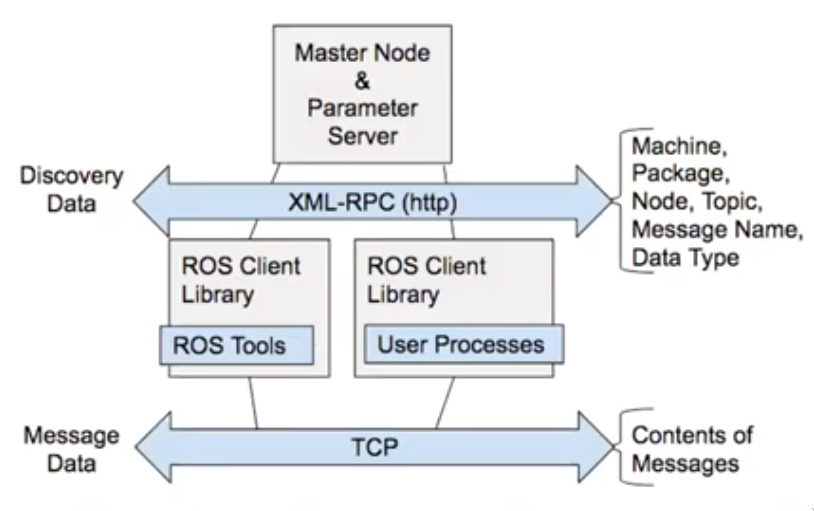
\includegraphics[width=0.6\linewidth]{images/former-ros1-architecture.png}
  \caption{Robot Operating System architecture.}
  \label{fig:ros1-architecture}
\end{figure}

Formerly, due to the sheer wide capabilities controlled by the master, this centralization approach was duly valorized. It naturally fits the purposes of a research tool, as it is simpler to monitor and analyze the system behaviour. However, because it is strongly reliant on the master node's availability, this communication architecture does not scale effectively, making it unsuitable for safety-critical or real-time applications. If the master fails, the entire system fails, representing a single point of failure and a huge performance bottleneck.

Many research communities tried to fix these real-time issues by proposing potential solutions, while supporting the same architecture design. Unfortunately, fell short of meeting the requirements of real-time applications. It became clear to the ROS community that the framework had architectural limitations that could not be rearranged using the same design approach \cite{maruyama2016exploring, dieber2020penetration}.

The \textit{Robot Operating System 2} comes as a complete refactoring of ROS, with the aim of increase the framework's real-time capabilities, by allowing the development of time-critical control over ROS, as it moves away from the former architectural design towards the implementation of an external middleware that can support the production needs of the outgrowing robotic systems \cite{kim2018security, casini2019response}.

\subsection{Data Distribution Service}

The \textit{Data Distributed System} (DDS) \cite{3} is an \textit{Object Management Group} (OMG) middleware standard. The standard was developed to address the demand for enhanced interoperability across different vendors' middleware frameworks, directly addressing data communication between nodes that belong to a \textit{publish-subscribe} communication architecture, for real-time and embedded systems. 

A communication middleware aims to ease the complexity behind creating and maintaining communication architectures. It is responsible for handling relevant aspects like network configuration, communication establishment, data sharing and low-level details. As a result, system developers can mainly focus on their applications purposes, rather than concerning about information moving across levels \cite{dds-what-is}. 

DDS uses the \textit{Data-Centric Publish Subscribe} (DCPS) model as its communication model approach. DCPS is based on a publish-subscribe pattern, where the \textit{data-centric} messaging technique is implemented. It conceptually creates a virtual \textit{Global Data Space}, acessible by any DDS-based application, where data is properly delivered to the applications which quest for it, saving bandwith and processing power \cite{3, pardo2005introduction}. A \textit{domain participant} enables an application to participate in the \textit{Global Data Space}, either as a \textit{publisher} or as a \textit{subscriber}, according to their role on data exchange \cite{maruyama2016exploring, alaerjan2017modeling, dcps-rtps}. 

\begin{figure}[H]
    \centering
    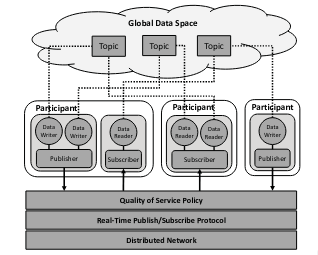
\includegraphics[width=0.4\linewidth]{images/dcps-model.png}
    \caption{DDS architecture: DCPS model with RTPS. Extracted from \cite{maruyama2016exploring}.}
    \label{fig:dcps-model}
\end{figure}

To properly address the data transportation through physical network, DDS offers a wire specification protocol called \textit{Real-Time Publish-Subscribe Wire Protocol} (RTPS) \cite{rtps}, providing automatic discovery between participants. This protocol also works under a publish-subscribe policy over best-effort transports, where data transmission between endpoints is handled \cite{yun2017data}. RTPS allows multiple applications, that could differ on their used DDS implementations, to interoperate with each other as network domain participants \cite{dcps-rtps, alaerjan2017modeling}.

Furthermore, RTPS was designed to employ \textit{Quality of Service} (QoS) profiles, which allow for the specification of various transport policies, formerly not covered by DDS. This approach offers flexibility over communication configuration and development versatility, allowing the developer to specify whatever QoS satisfies its system's communication needs \cite{alaerjan2017modeling, diluoffo2018robot, maruyama2016exploring}. 

Briefly, DDS leverages the premise of a transport-independent virtualized \textit{Data Bus} to address network resources' distribution, in which stateful data is distributed through the network. The involved applications can access this data in motion, representing an architecture with no single point of failure, respectively enabling a realiable way of ensuring data integrity. Consequently, by adopting this approach, the load on the network is independent of the number of applications, making it easily scalable.

\begin{figure}[H]
    \centering
    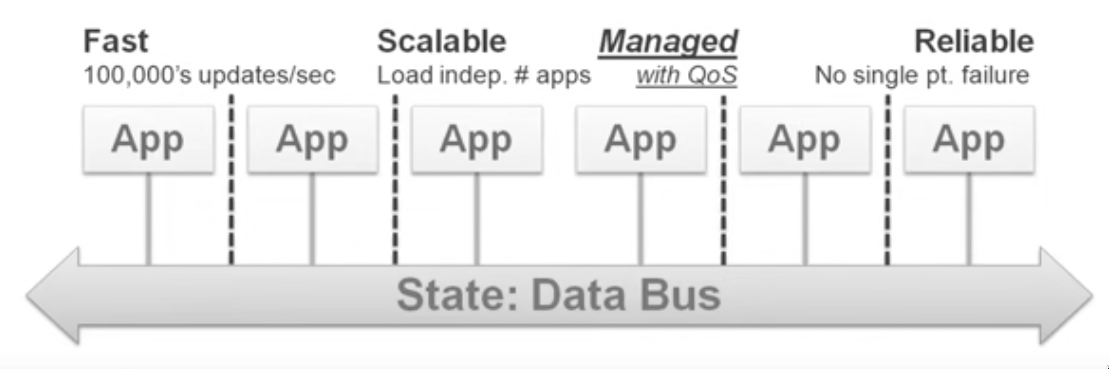
\includegraphics[width=0.6\linewidth]{images/dds-architecture.png}
    \caption{Data Distributed System architecture in a nutshell.}
    \label{fig:dds-architecture-nutshell}
\end{figure}


\subsection{ROS2-DDS Architecture}

As previously stated, the \textit{Robot Operating System 2} was developed to address the former architecture lack of support for real-time systems, mainly due to its architecture design that relied on their own middleware specification. To address this, ROS2 middleware approach is built upon the DDS framework \cite{maruyama2016exploring}, leveraging DDS for its messaging architecture, where communication and transport configuration are handled. 

As far as dependencies are concerned, DDS implementations have light sized dependencies, often related to language implementation libraries, easing the complexity behind installing and running dependencies \cite{ros-on-dds}.

The middleware's on-top layer regards the ROS client library (\textit{rcl}), already implemented in the former ROS architecture. This layer accounts the availability of ROS concepts to the Application layer, as it provides APIs to ease the software implementation by ROS developers \cite{ros2documentation}. As ROS aims to support different programming languages over the same computing context, each language-specficic API must have its corresponding client library (\textit{rclcpp} regarding \textit{C++} and \textit{rclpy} regarding \textit{Python}). The \textit{rcl} accounts these client libraries by abstracting their specification, consequently reducing code duplication \cite{rcl, casini2019response}.

\begin{figure}[H]
    \centering
    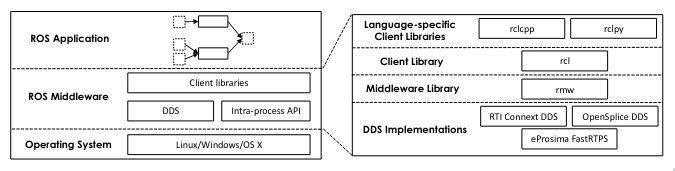
\includegraphics[width=\linewidth]{images/ros2-architecture.png}
    \caption{ROS2 framework architecture.}
    \label{fig:ros2-architecture}
\end{figure}

Towards supplying a wide range of configurations back to application layer, ROS2 aims to support multiple DDS implementations, in which these implementations API specification might differ from each other (currently, \textit{FastRTPS} by \textit{eProsima}, \textit{Connext} by \textit{RTI}, and \textit{Vortex OpenSplice} by \textit{Adlink}). It should be noted that the DDS implementations are low-level of abstraction, strictly defined by its corresponding vendor's API. DDS only defines fundamental procedures at a higher degree of abstraction.  

In order to abstract \textit{rcl} from the specifications complexity of these implementations APIs, an DDS-agnostic interface is being introduced, the \textit{rmw} (ROS MiddleWare) interface \cite{casini2019response}, allowing portability among DDS vendors, which consequently enables ROS developers to interpolate DDS implementations, based on their applications needs during runtime. The information flow through the middleware layer is done over structure mapping between ROS and DDS data models, addressed by the \textit{rmw}, regarding the DDS implementation that is being considered at runtime.

\subsection{Computation Graph}

From a logical perspective \cite{casini2019response}, ROS applications are composed of many software modules that operate as computation nodes, allowing its participation into the ROS \textit{Global Data Space}. The use of publish-subscribe model approach as communication type, through \textit{message-passing} patterns, confers additional concept complexity to the application architecture, where the latter can be naturally represented as a \textit{computation graph} \cite{cousins2010welcome}.

The application's computation graph presents itself as a graphical network, where runtime named entities have their unique role when it comes to data distribution.

\subsubsection{Node Instances}

The application development is done over package orchestrating, where each logically represents a useful software module. Packages might be compromised by numerous \textit{nodes}, that can be perceived as processes that will likely perform computation over the network. It is worth mentioning that, nodes can be connected within a single package or between multiple packages, as they are built over their corresponding packages \cite{cousins2010welcome, intro-ros}.

Thus, the network is comprised by many nodes, running simultaneously and exchanging data between them, where each node addresses its corresponding network module purpose \cite{ros2documentation}. Fault tolerance features are guaranteed as nodes have their corresponding unique name, allowing communication in an unambiguous manner, which confers a suitable approach when developing a complex robotic system.

The notable usage of callback functions provide great functionality when it comes to manage node's behaviour in the communication process. Additionally, \textit{timers} can also be used, since they provide a useful way of managing these callbacks, by time-assigning.

\subsubsection{Communication}

Message-passing is the primary means by which nodes communicate with one another. The \textit{message} definition is a well-typed data structure, which commonly characterizes every data structure concerning the information exchange between nodes. A message is defined by its data type, also known as its \textit{interface}, which can either be primitive (\textit{integer}, \textit{string}, \textit{boolean}, among others), or defined by a complex data structure, where multiple data types are assigned to their corresponding variables \cite{ros2documentation, intro-ros}.

ROS computation graph provides \textit{3} different ways of establish node communication, those being \textit{Topics}, \textit{Actions} and \textit{Services}. These communication mechanisms have different interfaces, specified in different folders with unique namespaces \cite{ros2documentation}.

The concrete mechanisms
\textit{Topics} are perhaps the most common method, naturally perceived as middle-communication buses, over which messages are passed through. As semantic approach, communication through topics is handled by the publishing-subscribing pattern. A node publishes the message to any number of topics, that are then subscribed by nodes that want to get access to that message. Topics provide a multicast routing scheme, where publish data is casted into the multiple nodes that are subscribed to the topic \cite{casini2019response}.

\begin{figure}[H]
    \centering
    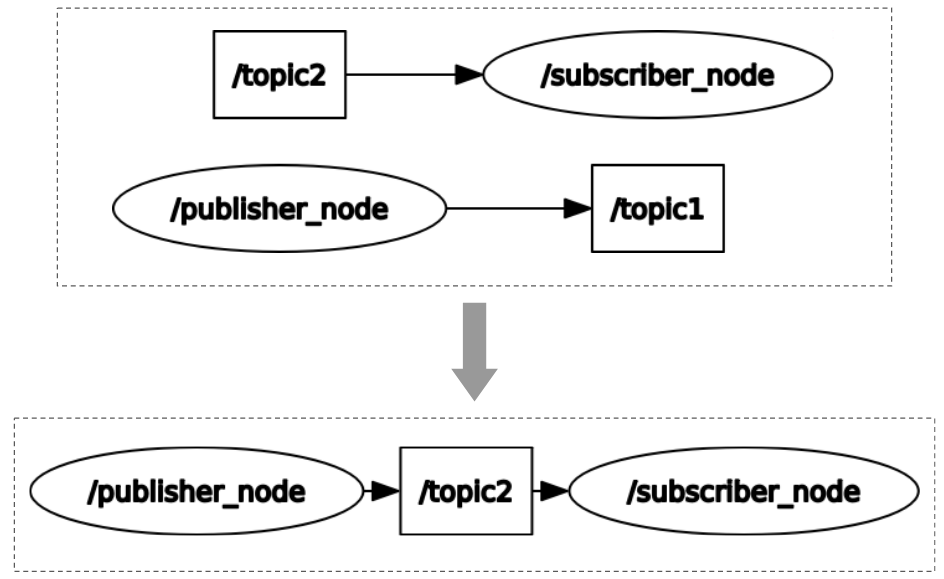
\includegraphics[width=0.5\linewidth]{images/ros2-topics.png}
    \caption{Communication behaviour over \textit{topics}.}
    \label{fig:ros2-topics}
\end{figure}

A specific \textit{topic} is created upon specifying its entity name over either a publisher or a subscriber callback instance. Whenever a node creates a publisher, intentionally instantiated to publish a message through a specified topic, \textit{roscore} is used to advertise the latter, enabling message passing to the corresponding topic subscribers. Message processing is done via the node's callback functions, which are activated upon message receipt, as it can also be utilized for publishing purposes \cite{casini2019response}.

Even though topics are the most conventional way of communication, due to its multicast scheme, subscribers can not be identified by the publishers, so logging and synchronization becomes rather difficult \cite{intro-ros}.

The use of \textit{services} enables a client node, that can also be seen as a topic subscriber, to request data from a server, that likewise a topic publisher, furnish data through a service. This is a bidirectional synchronous form of communication based on a request-response pattern.

Other notable way of exchanging data is by setting goals through \textit{Actions}. Actions are intended to process long-running tasks, where the client sends a goal request to the server node, that confirms the receiving of this goal. The server might provide feedback to the client before providing a response to the client. 


\subsubsection{Launch Files}

A conventional way of deploying a ROS application is through the use of \textit{launch files}, enabling the multi-configuration over entire robotic applications, where network nodes can be individually pre-configurated. Therefore, ROS makes use of the \textit{roslaunch} to automatically initialize the whole network, simultaneously launching each node \cite{intro-ros}. This provides a simpler way of monitoring the system nodes. 

The Figure \ref{fig:ts-rqt-graph} depicts the network architecture corresponding to an ROS application well-known example called the \textit{TurtleSim}. This application is mainly composed by \textit{two nodes}, that perform together towards moving a turtle. Additional nodes were implemented, in order to add complexity to the current network, as to later support security as a proper example. Briefly, the \textit{multiplexer} node acts as a topic selector between two different subscribed topics, where each of them was respectively associated with a priority value. Based on the priority valued, the \textit{multiplexer} node forwards the commands, related to the selected topic, into the \textit{turtlesim} node, triggering the turtle's movement. 

The \textit{rqt} \footnote[1]{ROS provides a GUI tool called \textit{rqt}, that assists developers in manipulating the network elements, in a more user-friendly manner.}, \textit{rqt\_graph}, allows the developer to perform analysis over a graphical visualization of the network computation graph.

\begin{figure}[H]
    \centering
    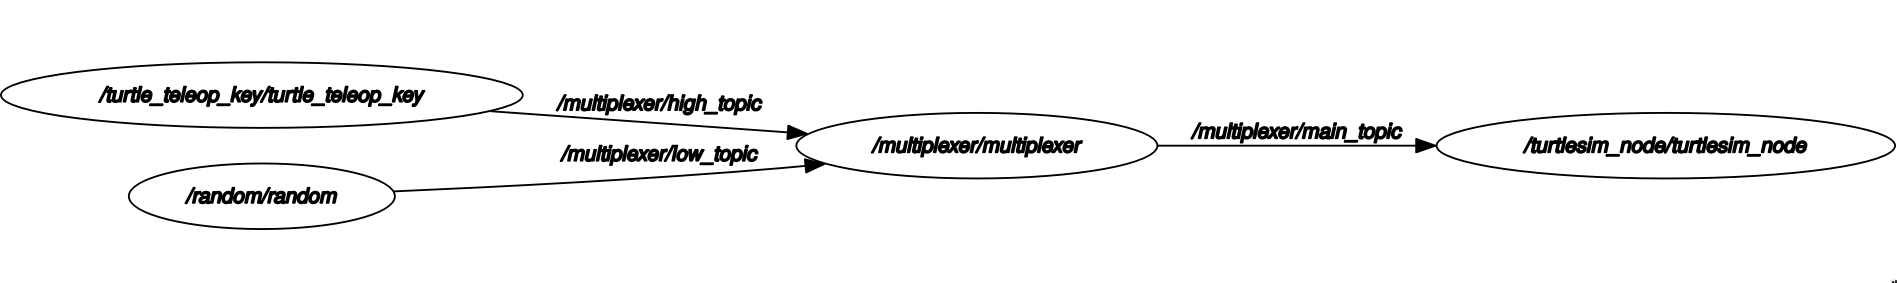
\includegraphics[width=0.8\linewidth]{images/ts_rqt_graph.png}
    \caption{\textit{TurtleSim}'s network graph presented by \textit{rqt\_graph}.}
    \label{fig:ts-rqt-graph}
\end{figure}

After the proper configuration of each node regarding the \textit{TurtleSim} example, the network can be easily managed and automatically launched through a launch file. The Figure \ref{fig:ros-lf} addresses the launch specification related to the latter application.

\begin{figure}[H]
\begin{lstlisting}[otherkeywords={launch, node, name, pkg, exec, output}]
<launch>
    <node name="turtlesim" pkg="default" exec="turtlesim" output="screen"/>
    <node name="keyboard" pkg="default" exec="keyboard"/>
    <node name="random" pkg="random" exec="random"/>
    <node name="multiplexer" pkg="multiplexer" exec="multiplexer"/>
</launch>
\end{lstlisting}
\caption{\textit{TurtleSim} launch file.}
\label{fig:ros-lf}
\end{figure}

Additional node configuration, such as name remapping and parameter adjustments, can be specified under the \textit{args} tag, which offers great functionality to the launching process. 

Distinctive namespaces allow the system to start the nodes, without any name nor topic name conflicts. However, this technique has some flaws attached, since it does not furnish a way of launching nodes in a separated terminal, often needed for user interaction purposes, like input reading.

\subsubsection{Parameters}   

Another relevant concept behind ROS is the existence of nodes \textit{parameters}, that allows individual configuration of the network nodes. In the former version of ROS, the node parameters were controlled by a global \textit{parameter server}, managed by its corresponding ROS Master \cite{intro-ros}. However, in ROS2 each node declares and manages its own parameters, by using the predefined commands \textit{get} and \textit{set}. Additionally, using a parameter function callback, the node's parameters can easily be edited \cite{ros2documentation}.
        
\subsubsection{Node Composition}  

Usually a node is attached to a single process, but it is possible to combine multiple nodes into a single process, structurally abstracting some network parts, while improving the network's performance \cite{ros2documentation}. However, there is a slight difference about how ROS and ROS2 approaches node composition. 

In the former version of ROS, node composition was done over the combination of \textit{nodelets}, intentionally designed to ease the cost of overusing TCP for message-passing between nodes \cite{ros-nodelets}.  Supported by the former idea of \textit{nodelets}, ROS2 introduces the \textit{components} as software code compiled into shared libraries, that can be loaded into a \textit{component container} process at runtime in the network, ensuring node composition \cite{ros2documentation}. 

%Node composition could also be applied for security matters. Suppose a scenario where multiple nodes respect the same security policies. By combining them into a single process, the mapping into this set of rules would be direct, easing the usage of security enclaves.
           

\section{Security}

The deployment of real-time systems implies critical concerning about safety and security \cite{maruyama2016exploring}, resulting of the demanding time-critical scenarios. 

Robotic systems fall under the umbrella of this broad system definition, as they feature unique cyber vulnerabilities related to its integration over highly networked environments, that confers great importance on exposing critical time-reliant scenarios \cite{mcclean2013preliminary, dieber2017security}.

\subsection{Former ROS Security Concerns}

The network security evaluation in a system is done by applying several analyzing techniques. Generally, these techniques do not cover every security aspect, as new vulnerabilities arise from technology evolution \cite{kaeo2004designing}.
The appliance of security countermeasures techniques upon configuring the system's network confers a critical step when aiming towards achieving security.

Within this vast topic, several avenues of endeavor come to mind, each deserving of a substantial study. Network security entails pre-exploration of the system's network through practical networking security techniques, such as intrusion detection and traffic analysis \cite{marin2005network}.

Numerous researchers \cite{8794451, dieber2020penetration} have investigated the use of these techniques, such as port scanning and penetration testing, over the previous version of ROS in order to thoroughly assess attack vulnerability throughout the ROS architecture. 

The ROS Master role in the communication architecture, and its ability to connect to other nodes, imposes many concerns about how to address security to ensure protection over the Master node. Exposing this node poses a critical threat over the whole network \cite{8794451}. 

Moreover, there were also worries regarding the way ROS handled node communication. Network security may be jeopardized, as a result of the publish-subscribe pattern transparency, where node-to-node communications are settled in plain text, making data content vulnerable to unauthorized usage \cite{kim2018security, white2016sros}. Additionally, the former API did not confer any message integrity technique, making applications vulnerable to packet sniffing and man-in-the-middle attacks \cite{white2016sros}.
 
However, due to the high non-linearity and complexity of real-time systems, implementing such thorough analysis method in near real-time remains a significant difficult task \cite{diao2009design}.

\subsection{DDS-Security Specification}

The \textit{Object Management Group} (OMG) \cite{3} accounts security integration by supplying an in-depth specification, consequently adding features to the already developed DDS standard. The \textit{DDS-Security} is a specification that serves as a security extension to the DDS protocol, defined by a set of plugins (Authentication, Access Control, Cryptographic, Logging, Data Tagging), combined in a \textit{Service Plugin Interface (SPI)} architecture \cite{8442103, ros-dds-integration}.

\begin{figure}[H]
    \centering
    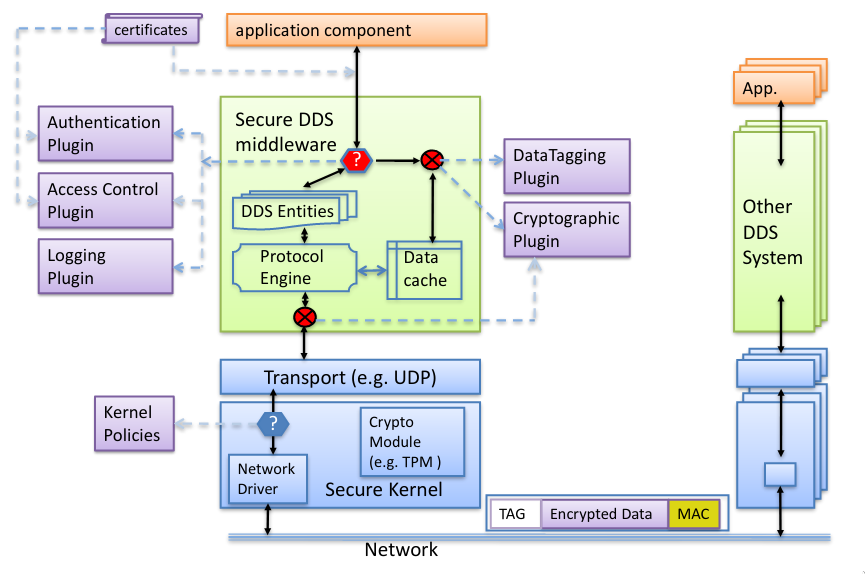
\includegraphics[width=0.7\linewidth]{images/dds-security-architecture.png}
    \caption{DDS-Security Architecture. Extracted from \cite{dds-s}.}
    \label{fig:dds-security-architecture}
\end{figure}

This specification enables its integration by furnishing a \textit{Security Model} supplied to the DDS standard, whereas the \textit{Service Plugin Interface} architecture is responsible for granting plugin enhancement for compliant DDS implementations. Moreover, depending on the security requirements needed for a particular application, these plugins might be adjusted by the latter's runtime DDS implementation \cite{dds-s}.

\subsubsection{Authentication}

Upon considering a secure environment over the DDS \textit{Global Data Space}, data integrity can not be prone to unauthorized usage. Therefore, data exchange requires verification procedures to properly identity the authenticity each DDS domain participant.

The Authentication plugin confers the most valued plugin to the entire SPI architecture, as it provides means to validate the identity of the application, later regarded as a domain participant \cite{dds-s, ros-dds-integration}. 

Each participant must be authenticated prior to entering the data space \cite{white2019network}. Therefore, participants are presented to the secured environment regarding the \textit{Public Key Infrastructure} (PKI). This latter is in charge of issuing asymmetric keys to each participant, a \textit{public} and \textit{private} key respectively, that are used for both authentication and encryption procedures \cite{diluoffo2018robot, ros-dds-integration}. 

Moreover, regarding the issuer identity, the PKI provides an \textit{X.509 certificate}, that maps a distinguished domain name (DN) to the participant's public key \cite{diluoffo2018robot, white2016sros}. This certificate is accountable and signed by a trusted certificate authority (CA) \cite{white2019network, white2016sros, ros-dds-integration}. It ensures authenticity between asymmetric key pairs (both \textit{public} and \textit{private}) \cite{diluoffo2018robot}. 

The communication establishment over different participants must be preceded by a mutual handshake, where keys and certificates are exchanged to guarantee their authenticity \cite{white2019network, kim2018security}. Additionally, the DDS permissions of a domain peer are also concerned within this handshake. The control over permission distribution is respectively handled by the Access Control plugin.

\subsubsection{Access Control}

As aforementioned, the defined DDS specification handles policy control over the DDS domain through the Access Control plugin, where authenticated parties respective operations are imposed by policy restrictions \cite{dds-s, white2019network}. Domains within the \textit{Global Data Space} are controlled over a set of DDS-related capabilities, that are either assigned or restricted to the authenticated participants \cite{ros-dds-integration}. 

Authenticated participants must be granted access to certain domains, where their roles on data transportation must be accordingly accounted by access permissions. If a participant is perceived as a domain data publisher, the domain restrictions must provide publishing privileges to its data topic \cite{white2019network}. 

Following the authentication procedure, domain authorization is also concerned using the proven PKI \cite{ros-dds-integration}, by embedding policy definitions through certificate extensions \cite{white2016sros}. 

Furthermore, the Access Control plugin employs \textit{2} configuration documents that are allocated to each participant \cite{white2019network}. This provides significant security capability, which is given as a supplement to the authentication procedure.

\textbullet\ Domain Governance: \textit{XML} document defining the domain's security policy.

\textbullet\ Participant Permissions: \textit{XML} document containing the permissions assigned to a given domain participant.

Notably, these configuration files are signed by a trusting Certificate Authority (CA) \cite{ros-dds-integration}. The CA's Permission Certificate confers protection against elevation of privilege attacks. Therefore, if the policy integrity is jeopardized, the handshake establishment between authenticated parties fails to commence \cite{white2016sros}.

\subsubsection{Communication and Encryption}

% The DDS-Security specification ensures encryption and authentication using \textit{OpenSSL}, while accounting security functions based on encryption standards \cite{takemoto2019performance}. Accordingly, it implements a handshake-based standard, concerning the \textit{OpenSSL} protocols, \textit{Secure Sockets Layer} (SSL) and \textit{Transport Layer Security} (TLS), which are used respectively used to ensure encryption over the network communication \cite{white2016sros, kim2018security}.

%The handshake is used to achieve mutual authentication within participants over the DDS domain. As stated, each participant must be authenticated prior to entering the data space \cite{white2019network}. Therefore, participants are presented to the secured environment regarding the Public Key Infrastructure (PKI). This latter is in charge of issuing a public certificate, accountable and signed by a trusted certificate authority (CA) \cite{white2019network, white2016sros}.

The DDS-Security specification ensures encryption and authentication using \textit{OpenSSL}, while accounting security functions based on encryption standards \cite{takemoto2019performance}. 

Accordingly, it implements a handshake-based standard, concerning the \textit{OpenSSL} protocols, \textit{Secure Sockets Layer} (SSL) and \textit{Transport Layer Security} (TLS), which are used respectively used to ensure encryption over the network communication \cite{white2016sros, kim2018security}. The handshake is used to achieve mutual authentication within participants over the DDS domain \cite{white2019network}.

Following the participant key assignment, the \textit{Diffie-Hellman} key exchange protocol properly accounts the mentioned handshake, allowing both participants to exchange data over a shared secret key \cite{kim2018security}. % while accounting their own public certificate information \cite{kim2018security}. 
It enjoys the inter-exchange of both asymmetric keys, issued to each domain participant during the domain authentication procedure, in order to perform sign (using the private key) and verify (using the public key) operations \cite{kim2018security, diluoffo2018robot}.

The \textit{rcl} is capable of handling this DDS security requirement, levering ROS-based applications to support SROS2, accounting nodes as authenticated participants \cite{white2016sros}. 

As communication establishment is duly achieved throughout this handshake process, the DDS-Security specification takes advantage of the \textit{AES-GCM} encryption standard concerning data encryption over the implicit channel \cite{kim2018security, takemoto2019performance}.

\begin{figure}[H]
    \centering
    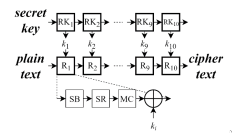
\includegraphics[width=0.4\linewidth]{images/ros_aes.png}
    \caption{\textit{Advanced Encryption Standard} algorithm. Extracted from \cite{takemoto2019performance}.}
    \label{fig:ros_aes}
\end{figure}

The \textit{key cryptosystem} algorithm \cite{takemoto2019performance} presented in the \textit{Advanced Encryption Standard (AES)} considers the usage of functions towards achieving data encryption over the established communication. It enables configuration over data encryption, allowing both block and streaming transfer of ciphered data \cite{diluoffo2018robot}.

Here, the algorithm combines the shared key established with the message passed over the secure channel. Moreover, it is desirable to implement the \textit{Galois MAC (AES-GMAC)} encryption algorithm, that is based on block cipher operations, consequently adding encryption functionality to the AES algorithm, through a \textit{Message Authentication Code (MAC)} encryption function \cite{takemoto2019performance, kim2018security}.

Every cryptography-related operations are handled by the SPI's Cryptographic plugin. Naturally, these cryptographic capabilities, linked to the asymmetric key cryptography, are then used by both Authentication and Access Control plugins, ensuring authenticity support over their corresponding opeartions \cite{ros-dds-integration, diluoffo2018robot}.

\subsection{Security Integration in ROS2}

As result of the \textit{Data Distribution Service} (DDS) implementation as a flexible middleware interface in the ROS2 architecture, issues regarding security is no longer mainly ROS-dependent. Thus, when it comes to addressing security over communication, and subsequently data protection enhancement, ROS2 is heavily reliant on how the DDS standard is able to manage security \cite{kim2018security, 8794451}.

Every DDS implementation supported by ROS2 makes use of the DDS-Security specification, enabling security over ROS's application environment. Even though ROS2 is deployed without security mechanisms by default \cite{ros-dds-integration}, ROS2 provides a toolset, the \textit{Secure Robot Operating System 2} (SROS2) toolset \cite{sros2-gh}, extending ROS2's functionality to make use of the DDS-Security functionality. 

The control over these tools are done by \textit{rcl}, providing security over the Application layer, while DDS is capable of providing security over the communication architecture \cite{kim2018security}. SROS2 configuration is done over applying a set of security files to each ROS2 participant, with regard to how DDS handles certificate assignment to their participants \cite{white2016sros, ros-dds-integration}. 

Consequently, the toolset allows certificate generation and allocation through a keyserver directory, where security enclaves and their respective authentication files are stored inside subfolders \cite{white2016sros, ros-dds-integration}. Moreover, SROS2 enables the keyserver configuration in a flexible way, allowing developers to restricit certificate and CA attributes to an arbitrary number of nodes, defined over the same namespace \cite{white2016sros}.

The variety of capabilities in SROS2 toolset attempts to aid with security configuration across environments \cite{ros-dds-integration}. However, managing certificates and access control policies might lead to improper configuration. Additionally, orchestrating a real-time network towards achieving a secure environment confers to be a demanding process \cite{ros-dds-integration, white2019network}.

% The SROS2 configuration is done over applying a set of security files to each ROS2 participant, with regard to how DDS handles certificate assignment to their participants \cite{white2016sros}. The variety of capabilities in SROS2 toolset attempts to aid with security configuration across environments, however, the developer must be aware of improper configuration, that can still lead to security problems \cite{ros-dds-integration}.

\subsubsection{Security Enclaves}

As aforementioned, ROS2 relies on how handles DDS security over their \textit{Domain Participants}. DDS imposes the authentication of each participant prior to joining its \textit{Global Data Space}, where the Certificate Authority and an established PKI comes in hand \cite{white2019network, white2016sros}.

Accordingly, the authentication process within the ROS2 network relies on the notion of a network enclave, where authentication and control artifacts are stored to properly achieve security over the network data space \cite{ros-security-enclaves}. Conceptually, an enclave is a secure region in the application address space that maintains confidentiality and integrity, while computations are being carried out on data.

Previously, a node was perceived as a separated DDS participant. However, by considering node composition as a reliable way of matching multiple nodes simultaneously to the same security domain, this node perception as participants can not be taken into account, due to causing non-negligible overhead, as memory space becomes rather difficult to handle \cite{ros-security-enclaves, ros-access-control}.

Concerning the enclave authentication procedure, its security artifacts must be addressable by a DDS participant, where the latter is associated to a node sharing context, instead of being perceived as a single node \cite{ros-security-enclaves}. Thus, when it comes to apply different policies over different nodes, that are matched in the same node context, a set of node \textit{profiles} can be specified under the enclave notation. 
 
\vspace{0.5cm}
\textbf{Access Control within Enclaves}

The SROS2 toolset offers a well-typed markup language \textit{XML schema} \cite{ros-access-control}, where security policies bind profiles to access permissions for network objects, granting privileges back to a certain profile. \textit{Profiles} are implemented under the \textit{enclave} declaration, to duly support the node composition into a single process, enabling the possibility of combining multiple profiles, respectively addressing its corresponding node. % Typically, each \textit{enclave} declaration is linked to a corresponding ROS node, naturally perceived as a DDS participant.

\textit{Objects} are classified over a subsystem type, structurally characterized by permissions tags. Then \textit{object privileges} are controlled over access values, either \textit{allow} or \textit{deny}, attributed to their corresponding permissions tags \cite{ros-access-control, white2018procedurally}. Briefly, each node profile is assigned to policies that concern some object identifier (OID). Each OID maps to a specific action, that is identified over an access value, allow or deny respectively \cite{white2016sros}.

The policy design approach works under the \textit{Mandatory Access Control} (MAC), that denies any privilege by default. The only way of allowing access to any object, is by explicitly specifying the subject's privilege access \cite{ros-access-control, white2018procedurally, white2016sros}. Naturally, this policy approach confers great value towards security, since it denies any attempt of privilege gaining attack by ROS-based packages from non-trusted sources \cite{white2016sros}.

Depicted in the Figure \ref{fig:ros-access-file}, it is presented a policy file where access control privileges are distributed across enclaves, and their inherited profiles. Recall the \textit{TurtleSim} example, the following \textit{XML} policy file addresses the access to topics for each respective enclave. 

\begin{figure}[H]
\begin{lstlisting}[otherkeywords = {xml, version, encoding, policy, version, enclave, enclaves, profile, profiles, topic, topics, xmlns:xi, path, ns, node, publish, subscribe, reply, request, call, execute, xi:include, href, xpointer}]
<?xml version="1.0" encoding="UTF-8"?>
<policy version="0.2.0" xmlns:xi="http://www.w3.org/2001/XInclude">
  <enclaves>
    <enclave path="/multiplexer">
      <profiles>
        <profile ns="/" node="multiplexer">
          <topics publish="ALLOW" >
            <topic>move_turtle</topic>
          </topics>
          <topics subscribe="ALLOW" >
            <topic>high_priority</topic>
            <topic>low_priority</topic>
          </topics>
        </profile>
      </profiles>
    </enclave>
    <enclave path="/turtlesim">
      <profiles>
        <profile ns="/" node="turtlesim">
          <topics subscribe="ALLOW" >
            <topic>move_turtle</topic>
          </topics>
        </profile>
      </profiles>
    </enclave>
    <enclave path="/keyboard">
      <profiles>
        <profile ns="/" node="keyboard">
          <topics publish="ALLOW" >
            <topic>high_priority</topic>
          </topics>
        </profile>
      </profiles>
    </enclave>
    <enclave path="/random">
      <profiles>
        <profile ns="/" node="random">
          <topics publish="ALLOW" >
            <topic>low_priority</topic>
          </topics>
        </profile>
      </profiles>
    </enclave>
  </enclaves>
</policy>
\end{lstlisting}
\caption{SROS2 policy file regarding the access control policies over the \textit{TurtleSim} example.}
\label{fig:ros-access-file}
\end{figure}

\chapter{Software Development in ROS2}\label{c:ros}

Robotic systems have emerged into several scenarios, where its usage ranges between basic processes automation, up to full performance over critical tasks, consequently causing the complexity increase in these domains. 

Due to the wide variety of robotic hardware presented in multiple domains, concerning about software development is rather difficult \cite{cousins2011exponential}. The reuse of code is non-trivial, and therefore, large-scale development is rendered untenable. The Robotic Operating System (ROS) presents itself as a middleware system, created to facilitate robotic system development in large scale.

In ROS, software flexibility was prioritized above all else, meaning that values like security were disregarded. Thus, ROS-based applications tend to face increased security risks, related to the exposure of the whole robotic network. Due to the scale and scope of the robotics growth, security insurance must be addressed as a developing priority \cite{diluoffo2018robot, kim2018security}.

The upgraded version of ROS, Robot Operating System 2 (ROS2), presents itself as a framework for developing robotic systems, supported by the Data Distribution Service (DDS) standard. Multiple middleware implementations are built over this standard, which provides numerous DDS-based specifications as well as valuable Quality of Service (QoS) transport parameters.

The DDS-Security specification \cite{dds-s} aims to supply multiple plugins regarding the security domain. Consequently, ROS2 yields a wider command toolset compared to the former version of ROS, as they bring forth to a toolset, the Secure Robot Operating System 2 (SROS2) toolset, concerning the security functionality that DDS-Security plugins offer.

This chapter introduces necessary background information over the major concepts on which this thesis rests. First, it is presented a detailed introduction to the concepts around Robot Operating System (ROS), as well as the evolution approach that ROS faced towards providing security to its deployed systems. Regarding this goal, Data Distribution Service (DDS) and its integration on Robot Operating System 2 (ROS2) must be contextualized beforehand.


\section{Architecture Considerations}

The Robot Operating System was created by a collaborative open-source community, that has undergone rapid development \cite{cousins2011exponential} to contribute in the advancement of cyber physical systems. It was purposefully designed to be a development enhancer for the realm of robotic applications \cite{diluoffo2018robot, intro-ros}.

Fundamentally, ROS is a middleware, as it provides a custom serialization format, a custom transport protocol as well as a custom central discovery mechanism, presenting itself as a distributed layer between the top application layer and the operating system layer. 

ROS was designed to provide as much as modularity and composability to the application layer as possible \cite{casini2019response}, allowing ROS applications to be built over several software modules, as independent computing processes called \textit{nodes}. These compose together to fulfill the deployment characteristics of the corresponding robot \cite{maruyama2016exploring}.

\subsection{Former Architecture}

The Robot Operating System architecture is based on a hybrid peer-to-peer implementation, where network communication is done over message-passing through a publish-subscribe pattern. The communication API relied on a stateless XML-encoded remote procedure protocol. Transport libraries regarded the data exchange accounting serialization over sockets \cite{white2016sros, dieber2020penetration}.

The architecture emphasized on approaching communication through a centralization perspective. It relied on the explicit implementation of a \textit{Master node}, that controlled every aspect of the communication establishment. Consequently, every information exchange within the network had to go through this master.


\begin{figure}[H]
  \centering
  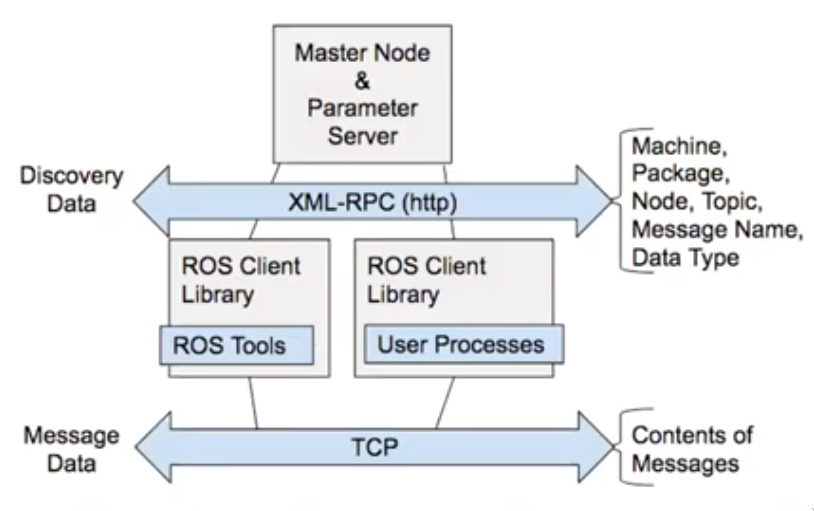
\includegraphics[width=0.6\linewidth]{images/former-ros1-architecture.png}
  \caption{Robot Operating System architecture.}
  \label{fig:ros1-architecture}
\end{figure}

Formerly, due to the sheer wide capabilities controlled by the master, this centralization approach was duly valorized. It naturally fits the purposes of a research tool, as it is simpler to monitor and analyze the system behaviour. However, because it is strongly reliant on the master node's availability, this communication architecture does not scale effectively, making it unsuitable for safety-critical or real-time applications. If the master fails, the entire system fails, representing a single point of failure and a huge performance bottleneck.

Many research communities tried to fix these real-time issues by proposing potential solutions, while supporting the same architecture design. Unfortunately, fell short of meeting the requirements of real-time applications. It became clear to the ROS community that the framework had architectural limitations that could not be rearranged using the same design approach \cite{maruyama2016exploring, dieber2020penetration}.

The \textit{Robot Operating System 2} comes as a complete refactoring of ROS, with the aim of increase the framework's real-time capabilities, by allowing the development of time-critical control over ROS, as it moves away from the former architectural design towards the implementation of an external middleware that can support the production needs of the outgrowing robotic systems \cite{kim2018security, casini2019response}.

\subsection{Data Distribution Service}

The \textit{Data Distributed System} (DDS) \cite{3} is an \textit{Object Management Group} (OMG) middleware standard. The standard was developed to address the demand for enhanced interoperability across different vendors' middleware frameworks, directly addressing data communication between nodes that belong to a \textit{publish-subscribe} communication architecture, for real-time and embedded systems. 

A communication middleware aims to ease the complexity behind creating and maintaining communication architectures. It is responsible for handling relevant aspects like network configuration, communication establishment, data sharing and low-level details. As a result, system developers can mainly focus on their applications purposes, rather than concerning about information moving across levels \cite{dds-what-is}. 

DDS uses the \textit{Data-Centric Publish Subscribe} (DCPS) model as its communication model approach. DCPS is based on a publish-subscribe pattern, where the \textit{data-centric} messaging technique is implemented. It conceptually creates a virtual \textit{Global Data Space}, acessible by any DDS-based application, where data is properly delivered to the applications which quest for it, saving bandwith and processing power \cite{3, pardo2005introduction}. A \textit{domain participant} enables an application to participate in the \textit{Global Data Space}, either as a \textit{publisher} or as a \textit{subscriber}, according to their role on data exchange \cite{maruyama2016exploring, alaerjan2017modeling, dcps-rtps}. 

\begin{figure}[H]
    \centering
    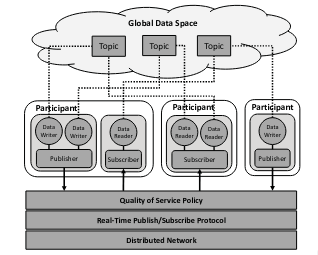
\includegraphics[width=0.4\linewidth]{images/dcps-model.png}
    \caption{DDS architecture: DCPS model with RTPS. Extracted from \cite{maruyama2016exploring}.}
    \label{fig:dcps-model}
\end{figure}

To properly address the data transportation through physical network, DDS offers a wire specification protocol called \textit{Real-Time Publish-Subscribe Wire Protocol} (RTPS) \cite{rtps}, providing automatic discovery between participants. This protocol also works under a publish-subscribe policy over best-effort transports, where data transmission between endpoints is handled \cite{yun2017data}. RTPS allows multiple applications, that could differ on their used DDS implementations, to interoperate with each other as network domain participants \cite{dcps-rtps, alaerjan2017modeling}.

Furthermore, RTPS was designed to employ \textit{Quality of Service} (QoS) profiles, which allow for the specification of various transport policies, formerly not covered by DDS. This approach offers flexibility over communication configuration and development versatility, allowing the developer to specify whatever QoS satisfies its system's communication needs \cite{alaerjan2017modeling, diluoffo2018robot, maruyama2016exploring}. 

Briefly, DDS leverages the premise of a transport-independent virtualized \textit{Data Bus} to address network resources' distribution, in which stateful data is distributed through the network. The involved applications can access this data in motion, representing an architecture with no single point of failure, respectively enabling a realiable way of ensuring data integrity. Consequently, by adopting this approach, the load on the network is independent of the number of applications, making it easily scalable.

\begin{figure}[H]
    \centering
    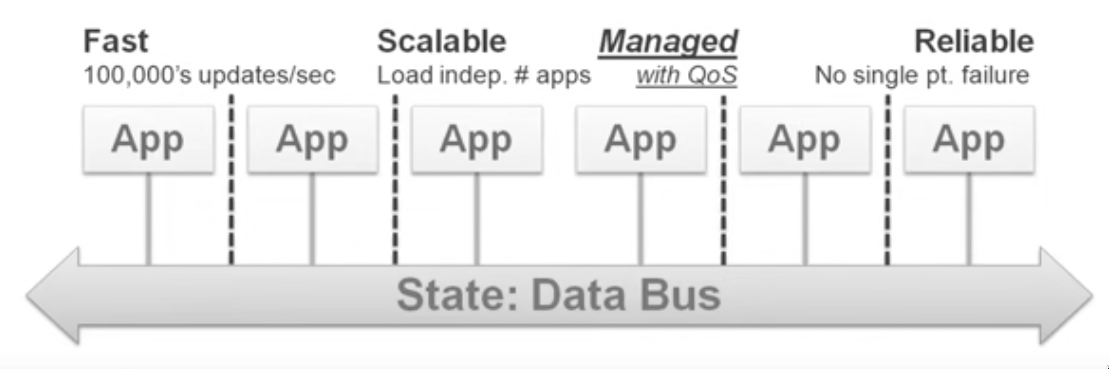
\includegraphics[width=0.6\linewidth]{images/dds-architecture.png}
    \caption{Data Distributed System architecture in a nutshell.}
    \label{fig:dds-architecture-nutshell}
\end{figure}


\subsection{ROS2-DDS Architecture}

As previously stated, the \textit{Robot Operating System 2} was developed to address the former architecture lack of support for real-time systems, mainly due to its architecture design that relied on their own middleware specification. To address this, ROS2 middleware approach is built upon the DDS framework \cite{maruyama2016exploring}, leveraging DDS for its messaging architecture, where communication and transport configuration are handled. 

As far as dependencies are concerned, DDS implementations have light sized dependencies, often related to language implementation libraries, easing the complexity behind installing and running dependencies \cite{ros-on-dds}.

The middleware's on-top layer regards the ROS client library (\textit{rcl}), already implemented in the former ROS architecture. This layer accounts the availability of ROS concepts to the Application layer, as it provides APIs to ease the software implementation by ROS developers \cite{ros2documentation}. As ROS aims to support different programming languages over the same computing context, each language-specficic API must have its corresponding client library (\textit{rclcpp} regarding \textit{C++} and \textit{rclpy} regarding \textit{Python}). The \textit{rcl} accounts these client libraries by abstracting their specification, consequently reducing code duplication \cite{rcl, casini2019response}.

\begin{figure}[H]
    \centering
    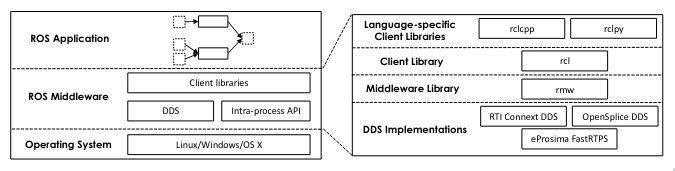
\includegraphics[width=\linewidth]{images/ros2-architecture.png}
    \caption{ROS2 framework architecture.}
    \label{fig:ros2-architecture}
\end{figure}

Towards supplying a wide range of configurations back to application layer, ROS2 aims to support multiple DDS implementations, in which these implementations API specification might differ from each other (currently, \textit{FastRTPS} by \textit{eProsima}, \textit{Connext} by \textit{RTI}, and \textit{Vortex OpenSplice} by \textit{Adlink}). It should be noted that the DDS implementations are low-level of abstraction, strictly defined by its corresponding vendor's API. DDS only defines fundamental procedures at a higher degree of abstraction.  

In order to abstract \textit{rcl} from the specifications complexity of these implementations APIs, an DDS-agnostic interface is being introduced, the \textit{rmw} (ROS MiddleWare) interface \cite{casini2019response}, allowing portability among DDS vendors, which consequently enables ROS developers to interpolate DDS implementations, based on their applications needs during runtime. The information flow through the middleware layer is done over structure mapping between ROS and DDS data models, addressed by the \textit{rmw}, regarding the DDS implementation that is being considered at runtime.

\subsection{Computation Graph}

From a logical perspective \cite{casini2019response}, ROS applications are composed of many software modules that operate as computation nodes, allowing its participation into the ROS \textit{Global Data Space}. The use of publish-subscribe model approach as communication type, through \textit{message-passing} patterns, confers additional concept complexity to the application architecture, where the latter can be naturally represented as a \textit{computation graph} \cite{cousins2010welcome}.

The application's computation graph presents itself as a graphical network, where runtime named entities have their unique role when it comes to data distribution.

\subsubsection{Node Instances}

The application development is done over package orchestrating, where each logically represents a useful software module. Packages might be compromised by numerous \textit{nodes}, that can be perceived as processes that will likely perform computation over the network. It is worth mentioning that, nodes can be connected within a single package or between multiple packages, as they are built over their corresponding packages \cite{cousins2010welcome, intro-ros}.

Thus, the network is comprised by many nodes, running simultaneously and exchanging data between them, where each node addresses its corresponding network module purpose \cite{ros2documentation}. Fault tolerance features are guaranteed as nodes have their corresponding unique name, allowing communication in an unambiguous manner, which confers a suitable approach when developing a complex robotic system.

The notable usage of callback functions provide great functionality when it comes to manage node's behaviour in the communication process. Additionally, \textit{timers} can also be used, since they provide a useful way of managing these callbacks, by time-assigning.

\subsubsection{Communication}

Message-passing is the primary means by which nodes communicate with one another. The \textit{message} definition is a well-typed data structure, which commonly characterizes every data structure concerning the information exchange between nodes. A message is defined by its data type, also known as its \textit{interface}, which can either be primitive (\textit{integer}, \textit{string}, \textit{boolean}, among others), or defined by a complex data structure, where multiple data types are assigned to their corresponding variables \cite{ros2documentation, intro-ros}.

ROS computation graph provides \textit{3} different ways of establish node communication, those being \textit{Topics}, \textit{Actions} and \textit{Services}. These communication mechanisms have different interfaces, specified in different folders with unique namespaces \cite{ros2documentation}.

The concrete mechanisms
\textit{Topics} are perhaps the most common method, naturally perceived as middle-communication buses, over which messages are passed through. As semantic approach, communication through topics is handled by the publishing-subscribing pattern. A node publishes the message to any number of topics, that are then subscribed by nodes that want to get access to that message. Topics provide a multicast routing scheme, where publish data is casted into the multiple nodes that are subscribed to the topic \cite{casini2019response}.

\begin{figure}[H]
    \centering
    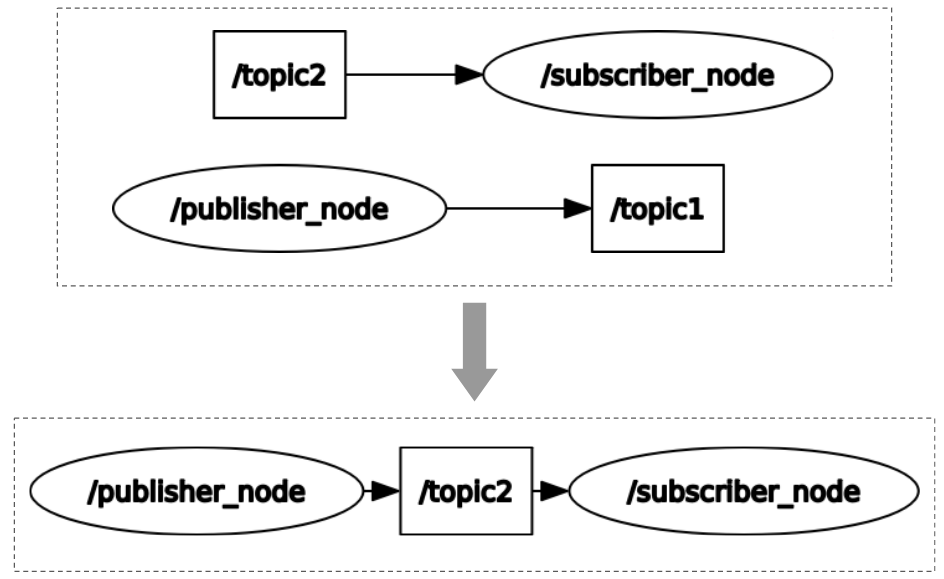
\includegraphics[width=0.5\linewidth]{images/ros2-topics.png}
    \caption{Communication behaviour over \textit{topics}.}
    \label{fig:ros2-topics}
\end{figure}

A specific \textit{topic} is created upon specifying its entity name over either a publisher or a subscriber callback instance. Whenever a node creates a publisher, intentionally instantiated to publish a message through a specified topic, \textit{roscore} is used to advertise the latter, enabling message passing to the corresponding topic subscribers. Message processing is done via the node's callback functions, which are activated upon message receipt, as it can also be utilized for publishing purposes \cite{casini2019response}.

Even though topics are the most conventional way of communication, due to its multicast scheme, subscribers can not be identified by the publishers, so logging and synchronization becomes rather difficult \cite{intro-ros}.

The use of \textit{services} enables a client node, that can also be seen as a topic subscriber, to request data from a server, that likewise a topic publisher, furnish data through a service. This is a bidirectional synchronous form of communication based on a request-response pattern.

Other notable way of exchanging data is by setting goals through \textit{Actions}. Actions are intended to process long-running tasks, where the client sends a goal request to the server node, that confirms the receiving of this goal. The server might provide feedback to the client before providing a response to the client. 


\subsubsection{Launch Files}

A conventional way of deploying a ROS application is through the use of \textit{launch files}, enabling the multi-configuration over entire robotic applications, where network nodes can be individually pre-configurated. Therefore, ROS makes use of the \textit{roslaunch} to automatically initialize the whole network, simultaneously launching each node \cite{intro-ros}. This provides a simpler way of monitoring the system nodes. 

The Figure \ref{fig:ts-rqt-graph} depicts the network architecture corresponding to an ROS application well-known example called the \textit{TurtleSim}. This application is mainly composed by \textit{two nodes}, that perform together towards moving a turtle. Additional nodes were implemented, in order to add complexity to the current network, as to later support security as a proper example. Briefly, the \textit{multiplexer} node acts as a topic selector between two different subscribed topics, where each of them was respectively associated with a priority value. Based on the priority valued, the \textit{multiplexer} node forwards the commands, related to the selected topic, into the \textit{turtlesim} node, triggering the turtle's movement. 

The \textit{rqt} \footnote[1]{ROS provides a GUI tool called \textit{rqt}, that assists developers in manipulating the network elements, in a more user-friendly manner.}, \textit{rqt\_graph}, allows the developer to perform analysis over a graphical visualization of the network computation graph.

\begin{figure}[H]
    \centering
    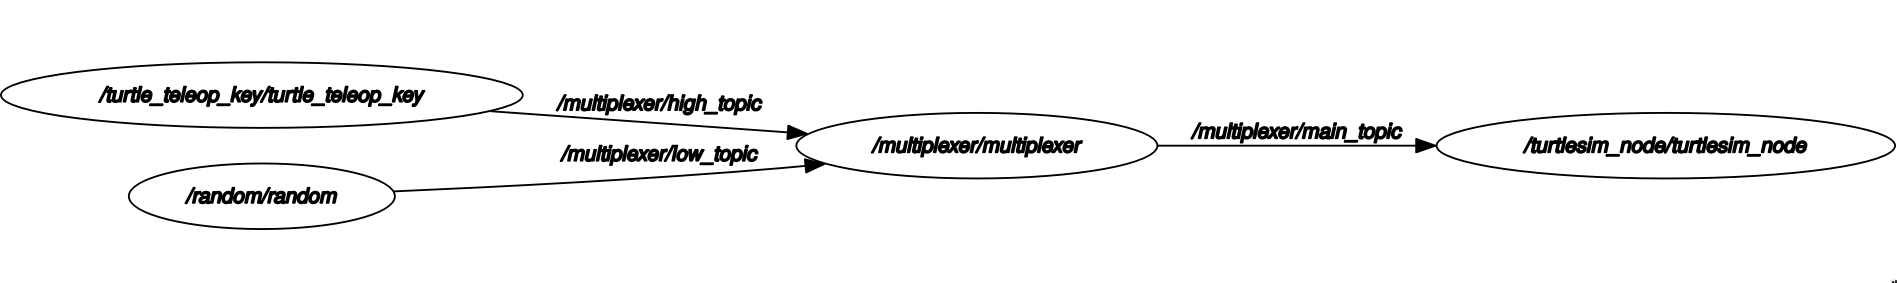
\includegraphics[width=0.8\linewidth]{images/ts_rqt_graph.png}
    \caption{\textit{TurtleSim}'s network graph presented by \textit{rqt\_graph}.}
    \label{fig:ts-rqt-graph}
\end{figure}

After the proper configuration of each node regarding the \textit{TurtleSim} example, the network can be easily managed and automatically launched through a launch file. The Figure \ref{fig:ros-lf} addresses the launch specification related to the latter application.

\begin{figure}[H]
\begin{lstlisting}[otherkeywords={launch, node, name, pkg, exec, output}]
<launch>
    <node name="turtlesim" pkg="default" exec="turtlesim" output="screen"/>
    <node name="keyboard" pkg="default" exec="keyboard"/>
    <node name="random" pkg="random" exec="random"/>
    <node name="multiplexer" pkg="multiplexer" exec="multiplexer"/>
</launch>
\end{lstlisting}
\caption{\textit{TurtleSim} launch file.}
\label{fig:ros-lf}
\end{figure}

Additional node configuration, such as name remapping and parameter adjustments, can be specified under the \textit{args} tag, which offers great functionality to the launching process. 

Distinctive namespaces allow the system to start the nodes, without any name nor topic name conflicts. However, this technique has some flaws attached, since it does not furnish a way of launching nodes in a separated terminal, often needed for user interaction purposes, like input reading.

\subsubsection{Parameters}   

Another relevant concept behind ROS is the existence of nodes \textit{parameters}, that allows individual configuration of the network nodes. In the former version of ROS, the node parameters were controlled by a global \textit{parameter server}, managed by its corresponding ROS Master \cite{intro-ros}. However, in ROS2 each node declares and manages its own parameters, by using the predefined commands \textit{get} and \textit{set}. Additionally, using a parameter function callback, the node's parameters can easily be edited \cite{ros2documentation}.
        
\subsubsection{Node Composition}  

Usually a node is attached to a single process, but it is possible to combine multiple nodes into a single process, structurally abstracting some network parts, while improving the network's performance \cite{ros2documentation}. However, there is a slight difference about how ROS and ROS2 approaches node composition. 

In the former version of ROS, node composition was done over the combination of \textit{nodelets}, intentionally designed to ease the cost of overusing TCP for message-passing between nodes \cite{ros-nodelets}.  Supported by the former idea of \textit{nodelets}, ROS2 introduces the \textit{components} as software code compiled into shared libraries, that can be loaded into a \textit{component container} process at runtime in the network, ensuring node composition \cite{ros2documentation}. 

%Node composition could also be applied for security matters. Suppose a scenario where multiple nodes respect the same security policies. By combining them into a single process, the mapping into this set of rules would be direct, easing the usage of security enclaves.
           

\section{Security}

The deployment of real-time systems implies critical concerning about safety and security \cite{maruyama2016exploring}, resulting of the demanding time-critical scenarios. 

Robotic systems fall under the umbrella of this broad system definition, as they feature unique cyber vulnerabilities related to its integration over highly networked environments, that confers great importance on exposing critical time-reliant scenarios \cite{mcclean2013preliminary, dieber2017security}.

\subsection{Former ROS Security Concerns}

The network security evaluation in a system is done by applying several analyzing techniques. Generally, these techniques do not cover every security aspect, as new vulnerabilities arise from technology evolution \cite{kaeo2004designing}.
The appliance of security countermeasures techniques upon configuring the system's network confers a critical step when aiming towards achieving security.

Within this vast topic, several avenues of endeavor come to mind, each deserving of a substantial study. Network security entails pre-exploration of the system's network through practical networking security techniques, such as intrusion detection and traffic analysis \cite{marin2005network}.

Numerous researchers \cite{8794451, dieber2020penetration} have investigated the use of these techniques, such as port scanning and penetration testing, over the previous version of ROS in order to thoroughly assess attack vulnerability throughout the ROS architecture. 

The ROS Master role in the communication architecture, and its ability to connect to other nodes, imposes many concerns about how to address security to ensure protection over the Master node. Exposing this node poses a critical threat over the whole network \cite{8794451}. 

Moreover, there were also worries regarding the way ROS handled node communication. Network security may be jeopardized, as a result of the publish-subscribe pattern transparency, where node-to-node communications are settled in plain text, making data content vulnerable to unauthorized usage \cite{kim2018security, white2016sros}. Additionally, the former API did not confer any message integrity technique, making applications vulnerable to packet sniffing and man-in-the-middle attacks \cite{white2016sros}.
 
However, due to the high non-linearity and complexity of real-time systems, implementing such thorough analysis method in near real-time remains a significant difficult task \cite{diao2009design}.

\subsection{DDS-Security Specification}

The \textit{Object Management Group} (OMG) \cite{3} accounts security integration by supplying an in-depth specification, consequently adding features to the already developed DDS standard. The \textit{DDS-Security} is a specification that serves as a security extension to the DDS protocol, defined by a set of plugins (Authentication, Access Control, Cryptographic, Logging, Data Tagging), combined in a \textit{Service Plugin Interface (SPI)} architecture \cite{8442103, ros-dds-integration}.

\begin{figure}[H]
    \centering
    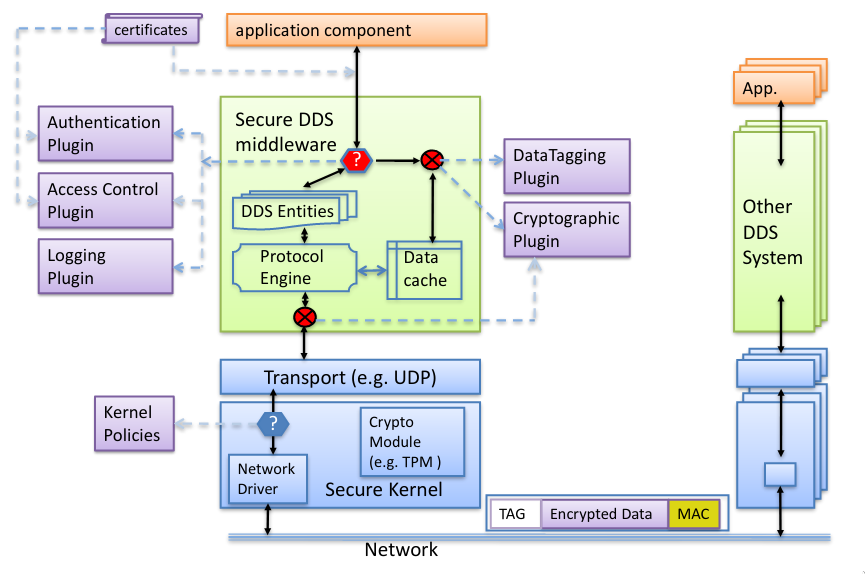
\includegraphics[width=0.7\linewidth]{images/dds-security-architecture.png}
    \caption{DDS-Security Architecture. Extracted from \cite{dds-s}.}
    \label{fig:dds-security-architecture}
\end{figure}

This specification enables its integration by furnishing a \textit{Security Model} supplied to the DDS standard, whereas the \textit{Service Plugin Interface} architecture is responsible for granting plugin enhancement for compliant DDS implementations. Moreover, depending on the security requirements needed for a particular application, these plugins might be adjusted by the latter's runtime DDS implementation \cite{dds-s}.

\subsubsection{Authentication}

Upon considering a secure environment over the DDS \textit{Global Data Space}, data integrity can not be prone to unauthorized usage. Therefore, data exchange requires verification procedures to properly identity the authenticity each DDS domain participant.

The Authentication plugin confers the most valued plugin to the entire SPI architecture, as it provides means to validate the identity of the application, later regarded as a domain participant \cite{dds-s, ros-dds-integration}. 

Each participant must be authenticated prior to entering the data space \cite{white2019network}. Therefore, participants are presented to the secured environment regarding the \textit{Public Key Infrastructure} (PKI). This latter is in charge of issuing asymmetric keys to each participant, a \textit{public} and \textit{private} key respectively, that are used for both authentication and encryption procedures \cite{diluoffo2018robot, ros-dds-integration}. 

Moreover, regarding the issuer identity, the PKI provides an \textit{X.509 certificate}, that maps a distinguished domain name (DN) to the participant's public key \cite{diluoffo2018robot, white2016sros}. This certificate is accountable and signed by a trusted certificate authority (CA) \cite{white2019network, white2016sros, ros-dds-integration}. It ensures authenticity between asymmetric key pairs (both \textit{public} and \textit{private}) \cite{diluoffo2018robot}. 

The communication establishment over different participants must be preceded by a mutual handshake, where keys and certificates are exchanged to guarantee their authenticity \cite{white2019network, kim2018security}. Additionally, the DDS permissions of a domain peer are also concerned within this handshake. The control over permission distribution is respectively handled by the Access Control plugin.

\subsubsection{Access Control}

As aforementioned, the defined DDS specification handles policy control over the DDS domain through the Access Control plugin, where authenticated parties respective operations are imposed by policy restrictions \cite{dds-s, white2019network}. Domains within the \textit{Global Data Space} are controlled over a set of DDS-related capabilities, that are either assigned or restricted to the authenticated participants \cite{ros-dds-integration}. 

Authenticated participants must be granted access to certain domains, where their roles on data transportation must be accordingly accounted by access permissions. If a participant is perceived as a domain data publisher, the domain restrictions must provide publishing privileges to its data topic \cite{white2019network}. 

Following the authentication procedure, domain authorization is also concerned using the proven PKI \cite{ros-dds-integration}, by embedding policy definitions through certificate extensions \cite{white2016sros}. 

Furthermore, the Access Control plugin employs \textit{2} configuration documents that are allocated to each participant \cite{white2019network}. This provides significant security capability, which is given as a supplement to the authentication procedure.

\textbullet\ Domain Governance: \textit{XML} document defining the domain's security policy.

\textbullet\ Participant Permissions: \textit{XML} document containing the permissions assigned to a given domain participant.

Notably, these configuration files are signed by a trusting Certificate Authority (CA) \cite{ros-dds-integration}. The CA's Permission Certificate confers protection against elevation of privilege attacks. Therefore, if the policy integrity is jeopardized, the handshake establishment between authenticated parties fails to commence \cite{white2016sros}.

\subsubsection{Communication and Encryption}

% The DDS-Security specification ensures encryption and authentication using \textit{OpenSSL}, while accounting security functions based on encryption standards \cite{takemoto2019performance}. Accordingly, it implements a handshake-based standard, concerning the \textit{OpenSSL} protocols, \textit{Secure Sockets Layer} (SSL) and \textit{Transport Layer Security} (TLS), which are used respectively used to ensure encryption over the network communication \cite{white2016sros, kim2018security}.

%The handshake is used to achieve mutual authentication within participants over the DDS domain. As stated, each participant must be authenticated prior to entering the data space \cite{white2019network}. Therefore, participants are presented to the secured environment regarding the Public Key Infrastructure (PKI). This latter is in charge of issuing a public certificate, accountable and signed by a trusted certificate authority (CA) \cite{white2019network, white2016sros}.

The DDS-Security specification ensures encryption and authentication using \textit{OpenSSL}, while accounting security functions based on encryption standards \cite{takemoto2019performance}. 

Accordingly, it implements a handshake-based standard, concerning the \textit{OpenSSL} protocols, \textit{Secure Sockets Layer} (SSL) and \textit{Transport Layer Security} (TLS), which are used respectively used to ensure encryption over the network communication \cite{white2016sros, kim2018security}. The handshake is used to achieve mutual authentication within participants over the DDS domain \cite{white2019network}.

Following the participant key assignment, the \textit{Diffie-Hellman} key exchange protocol properly accounts the mentioned handshake, allowing both participants to exchange data over a shared secret key \cite{kim2018security}. % while accounting their own public certificate information \cite{kim2018security}. 
It enjoys the inter-exchange of both asymmetric keys, issued to each domain participant during the domain authentication procedure, in order to perform sign (using the private key) and verify (using the public key) operations \cite{kim2018security, diluoffo2018robot}.

The \textit{rcl} is capable of handling this DDS security requirement, levering ROS-based applications to support SROS2, accounting nodes as authenticated participants \cite{white2016sros}. 

As communication establishment is duly achieved throughout this handshake process, the DDS-Security specification takes advantage of the \textit{AES-GCM} encryption standard concerning data encryption over the implicit channel \cite{kim2018security, takemoto2019performance}.

\begin{figure}[H]
    \centering
    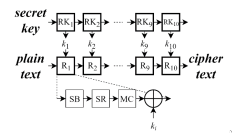
\includegraphics[width=0.4\linewidth]{images/ros_aes.png}
    \caption{\textit{Advanced Encryption Standard} algorithm. Extracted from \cite{takemoto2019performance}.}
    \label{fig:ros_aes}
\end{figure}

The \textit{key cryptosystem} algorithm \cite{takemoto2019performance} presented in the \textit{Advanced Encryption Standard (AES)} considers the usage of functions towards achieving data encryption over the established communication. It enables configuration over data encryption, allowing both block and streaming transfer of ciphered data \cite{diluoffo2018robot}.

Here, the algorithm combines the shared key established with the message passed over the secure channel. Moreover, it is desirable to implement the \textit{Galois MAC (AES-GMAC)} encryption algorithm, that is based on block cipher operations, consequently adding encryption functionality to the AES algorithm, through a \textit{Message Authentication Code (MAC)} encryption function \cite{takemoto2019performance, kim2018security}.

Every cryptography-related operations are handled by the SPI's Cryptographic plugin. Naturally, these cryptographic capabilities, linked to the asymmetric key cryptography, are then used by both Authentication and Access Control plugins, ensuring authenticity support over their corresponding opeartions \cite{ros-dds-integration, diluoffo2018robot}.

\subsection{Security Integration in ROS2}

As result of the \textit{Data Distribution Service} (DDS) implementation as a flexible middleware interface in the ROS2 architecture, issues regarding security is no longer mainly ROS-dependent. Thus, when it comes to addressing security over communication, and subsequently data protection enhancement, ROS2 is heavily reliant on how the DDS standard is able to manage security \cite{kim2018security, 8794451}.

Every DDS implementation supported by ROS2 makes use of the DDS-Security specification, enabling security over ROS's application environment. Even though ROS2 is deployed without security mechanisms by default \cite{ros-dds-integration}, ROS2 provides a toolset, the \textit{Secure Robot Operating System 2} (SROS2) toolset \cite{sros2-gh}, extending ROS2's functionality to make use of the DDS-Security functionality. 

The control over these tools are done by \textit{rcl}, providing security over the Application layer, while DDS is capable of providing security over the communication architecture \cite{kim2018security}. SROS2 configuration is done over applying a set of security files to each ROS2 participant, with regard to how DDS handles certificate assignment to their participants \cite{white2016sros, ros-dds-integration}. 

Consequently, the toolset allows certificate generation and allocation through a keyserver directory, where security enclaves and their respective authentication files are stored inside subfolders \cite{white2016sros, ros-dds-integration}. Moreover, SROS2 enables the keyserver configuration in a flexible way, allowing developers to restricit certificate and CA attributes to an arbitrary number of nodes, defined over the same namespace \cite{white2016sros}.

The variety of capabilities in SROS2 toolset attempts to aid with security configuration across environments \cite{ros-dds-integration}. However, managing certificates and access control policies might lead to improper configuration. Additionally, orchestrating a real-time network towards achieving a secure environment confers to be a demanding process \cite{ros-dds-integration, white2019network}.

% The SROS2 configuration is done over applying a set of security files to each ROS2 participant, with regard to how DDS handles certificate assignment to their participants \cite{white2016sros}. The variety of capabilities in SROS2 toolset attempts to aid with security configuration across environments, however, the developer must be aware of improper configuration, that can still lead to security problems \cite{ros-dds-integration}.

\subsubsection{Security Enclaves}

As aforementioned, ROS2 relies on how handles DDS security over their \textit{Domain Participants}. DDS imposes the authentication of each participant prior to joining its \textit{Global Data Space}, where the Certificate Authority and an established PKI comes in hand \cite{white2019network, white2016sros}.

Accordingly, the authentication process within the ROS2 network relies on the notion of a network enclave, where authentication and control artifacts are stored to properly achieve security over the network data space \cite{ros-security-enclaves}. Conceptually, an enclave is a secure region in the application address space that maintains confidentiality and integrity, while computations are being carried out on data.

Previously, a node was perceived as a separated DDS participant. However, by considering node composition as a reliable way of matching multiple nodes simultaneously to the same security domain, this node perception as participants can not be taken into account, due to causing non-negligible overhead, as memory space becomes rather difficult to handle \cite{ros-security-enclaves, ros-access-control}.

Concerning the enclave authentication procedure, its security artifacts must be addressable by a DDS participant, where the latter is associated to a node sharing context, instead of being perceived as a single node \cite{ros-security-enclaves}. Thus, when it comes to apply different policies over different nodes, that are matched in the same node context, a set of node \textit{profiles} can be specified under the enclave notation. 
 
\vspace{0.5cm}
\textbf{Access Control within Enclaves}

The SROS2 toolset offers a well-typed markup language \textit{XML schema} \cite{ros-access-control}, where security policies bind profiles to access permissions for network objects, granting privileges back to a certain profile. \textit{Profiles} are implemented under the \textit{enclave} declaration, to duly support the node composition into a single process, enabling the possibility of combining multiple profiles, respectively addressing its corresponding node. % Typically, each \textit{enclave} declaration is linked to a corresponding ROS node, naturally perceived as a DDS participant.

\textit{Objects} are classified over a subsystem type, structurally characterized by permissions tags. Then \textit{object privileges} are controlled over access values, either \textit{allow} or \textit{deny}, attributed to their corresponding permissions tags \cite{ros-access-control, white2018procedurally}. Briefly, each node profile is assigned to policies that concern some object identifier (OID). Each OID maps to a specific action, that is identified over an access value, allow or deny respectively \cite{white2016sros}.

The policy design approach works under the \textit{Mandatory Access Control} (MAC), that denies any privilege by default. The only way of allowing access to any object, is by explicitly specifying the subject's privilege access \cite{ros-access-control, white2018procedurally, white2016sros}. Naturally, this policy approach confers great value towards security, since it denies any attempt of privilege gaining attack by ROS-based packages from non-trusted sources \cite{white2016sros}.

Depicted in the Figure \ref{fig:ros-access-file}, it is presented a policy file where access control privileges are distributed across enclaves, and their inherited profiles. Recall the \textit{TurtleSim} example, the following \textit{XML} policy file addresses the access to topics for each respective enclave. 

\begin{figure}[H]
\begin{lstlisting}[otherkeywords = {xml, version, encoding, policy, version, enclave, enclaves, profile, profiles, topic, topics, xmlns:xi, path, ns, node, publish, subscribe, reply, request, call, execute, xi:include, href, xpointer}]
<?xml version="1.0" encoding="UTF-8"?>
<policy version="0.2.0" xmlns:xi="http://www.w3.org/2001/XInclude">
  <enclaves>
    <enclave path="/multiplexer">
      <profiles>
        <profile ns="/" node="multiplexer">
          <topics publish="ALLOW" >
            <topic>move_turtle</topic>
          </topics>
          <topics subscribe="ALLOW" >
            <topic>high_priority</topic>
            <topic>low_priority</topic>
          </topics>
        </profile>
      </profiles>
    </enclave>
    <enclave path="/turtlesim">
      <profiles>
        <profile ns="/" node="turtlesim">
          <topics subscribe="ALLOW" >
            <topic>move_turtle</topic>
          </topics>
        </profile>
      </profiles>
    </enclave>
    <enclave path="/keyboard">
      <profiles>
        <profile ns="/" node="keyboard">
          <topics publish="ALLOW" >
            <topic>high_priority</topic>
          </topics>
        </profile>
      </profiles>
    </enclave>
    <enclave path="/random">
      <profiles>
        <profile ns="/" node="random">
          <topics publish="ALLOW" >
            <topic>low_priority</topic>
          </topics>
        </profile>
      </profiles>
    </enclave>
  </enclaves>
</policy>
\end{lstlisting}
\caption{SROS2 policy file regarding the access control policies over the \textit{TurtleSim} example.}
\label{fig:ros-access-file}
\end{figure}

%\chapter{Verification of Information-Flow Properties concerning Security}\label{c:currWork}
\chapter{State of the Art}\label{c:currWork}

\section{Related work}\label{s:relWork}

This section intends to present previous developed work regarding the main concepts on what this dissertation rests. The subsection \ref{s:relWork-sec} aims to provide a comprehensive overview over works that attended to prevent security issues related to the deployment of robotic systems using Robot Operating System, as its application enhancer. It is then followed by the subsection % \ref{s:relWork-sa} regarding some of the current static analysis approaches on ROS applications. The latter subsection 
\ref{s:relWork-pv} that concerns about previous work addressing property verification and model checking techniques over ROS applications.

\subsection{Security Overview}\label{s:relWork-sec}

% This section aims to present previous works that attended security matters related to the deployment of robotic systems using Robot Operating System as its application enhancer. When developing real-time systems, safety matters are often referred as critical, because of the overall integration with the real world. Security however, it is measured by evaluating different security issues by properly analysing the system model. However, due to the high nonlinearity and complexity of real-time systems, implementing such a thorough analysis method in near real-time remains a significant difficulty. \cite{diao2009design}

% The deployment of real-time systems results in the importance of concerning about safety in a performance point of view, resulting of the demanding time-critical scenarios. Many studies were made regarding the performance in both ROS and ROS2 (also regarding DDS Quality of Service policies \cite{maruyama2016exploring}), by analysing using performance measurement approaches, providing a guided and supported review on how performance can directly affect time critical situations, where safety is envolved. \cite{maruyama2016exploring, casini2019response} 

% System security concerning network exposure, often explored by unauthorized acess and data leaking, can be treacherous and it is considered a complex subject, due to the abundance of different network security technologies that do not cover every security aspect, since absolute security does not exist, as new vulnerabilites arise from the tecnology evolution.\cite{kaeo2004designing} The creation and deployment of security countermeasures are essential upon configurating the network towards achieving security. Within this vast topic, several different avenues of endeavor come to mind, each deserving of a substantial study. Network security means exploring the network beforehand by computer intrusion detection, traffic analysis, network monitoring, alongside many other practical networking security aspects. \cite{marin2005network}

The literature concerning the network security enhancment that Robot Operating System 2 furnishes, by offering the SROS2 toolset, is quite limited. Most of the existing work is on the exploration of the former version of ROS in terms of port exposure, contextualized in the approach considered to protect the system network.  

Many researches were made regarding this issue that ROS faces, one in particular that explored the IPv4 address space of the Internet for instances of ROS, named \textit{Scanning the Internet for ROS: A View of Security in Robotics Research} \cite{8794451}, with the goal of identifying ROS vulnerable hosts, mostly master nodes since they provide information about their related topics and node's parameters, mainly by port scanning, so that developers could be aware of the possibility of exposure of their robots. % The performed scans furnished information about hosts that could either be a sensor, an actuator or even a simulator. Topics were also identified since they provide evidence of what is likely to be available to an attacker. This study is rather relevant because of how easily can attackers gather information about potential robots, and control them further on, through the public Internet, making it unavoidable to develop mechanisms concerning security.

Following the need of supplying security assurance over ROS applications, several approaches were presented. A study that is rather relevant because of the similarity between their proposal and the one that SROS2 has to offer is the one presented on the \textit{Application-level security for ROS-based applications} \cite{application-security-ros}. The approach primarily focused on applying security measures on the application layer, by mainly running an Authentication Server, storing certificates and files related to trusted domain participants, while controlling and providing session keys related to the communication process. Even though encryption and authentication measures are concerned, the protected network is still perceived from the "outside", meaning that security attacks, such as denial of service, still persist which cannot be handled on the application level alone. Secure Robot Operating System (SROS) \cite{white2016sros} was initially developed as an experimental tool (later evolved to SROS2 as a supporting tool for ROS2), which supports TLS for all socket transport, node restrictions and chains of trust, guaranteeing publishers authorization when it comes to publish to a specific topic. Another worth-mentioned tool is Rosbridge \cite{crick2017rosbridge}, which provides a WebSocket interface to ROS and corresponding server to allow interaction between applications and ROS nodes, by using TLS as support and also access control over topics and API calls. 

The present works addressing ROS security methods tend to concern solutions to prevent vulnerabilites and issues that might compromise robotic applications deployed, while considering performance as priority. In terms of applying formal methods to verify properties regarding the domain of ROS2 and ROS2 security as models, there are minimal existent works. Despite this, the following section consists of several articles proposed to validate robotic systems, using formal methods as core.

% \subsection{Static Analysis}\label{s:relWork-sa}

\subsection{Analysis and Verification}\label{s:relWork-pv}

Static analysis over ROS represents a major contribution to this domain, in which researchers aim to tackle issues arised from miss configurations or code inconsistencies. The noteworthy \textit{HAROS} framework \cite{santos2016framework} holds great value thanks to its contribution on improving ROS's software quality. \textit{HAROS} makes use of several analysis techniques to exert quality evaluation of ROS software, followed by ways of feedbacking inconsistencies using predefined code metrics. As this framework seeks to be flexible when it comes to adding functionality, further static analysis works improvements have been proposed as plugins. In both \citenum{santos2019static} and \citenum{santos2018property}, it is presented additional functionality to the framework, through applying architectural considerations over metamodel designing, where the latter supports the former by supplying property-based specifications. These techniques confers great help back to developers, since static analysis offers advantageable usage over raw review of software code. 

The literature concerning property verification over model checking tools is quite extensive. Regarding ROS applications, some approaches were presented that mainly focused on modelling the ROS node-communication, while real-time properties were also considered as support to the target language. In \citenum{halder2017formal}, \textit{UPPAAL} model checker is used to model ROS applications, supported by a concrete robot example, that is followed by techniques to verify properties regarding its behaviour. In \citenum{9341085} is presented a notable proposal, where \textit{Electrum} \cite{lwspecification}, the former version of the current Alloy Analyzer, is used as an additional plug-in to the already mentioned \textit{HAROS} framework. Through ROS launch configurations, the plugin automatically generated models using Electrum and performs verification over these models, to then feedback issues related to their ROS system behaviour.

As ROS2 domain regards the use of DDS communication protocol, a few works on DDS modelling analysis deserve to be mentioned, as they might give important background for property verification over communications protocols. In \citenum{alaerjan2017modeling}, it is proposed a technique to model the DCPS architectural design that DDS makes use of, alongside with new approaches to the current DDS behaviour. Supported by several modelling techniques for publish-subscribe systems, in \citenum{liu2018formal}, DDS in ROS2 is formalized as a timed automata, consequently followed by model verification over property-checking. These works conceive value concepts and procedures useful for this dissertation contextualization.

A few studies on robotics should be recognized in which techniques such as model-checking were performed. Despite the fact that they do not address the domain of ROS, they nonetheless give helpful background for the robotics research over formal approaches. A case study, mentioned in \citenum{near2011lightweight}, presents a novel approach over systems that require static analysis based on software assumptions and proper analysis within its environment usage, where user-interaction comes in hand. Concerning this novel idea, a medical system is concerned as a case study, where multiple safety-based considerations are expected, as well as, an end-to-end critical property that must be satisfied over the entire analysis course. Another notable work regarding former analysis using Alloy specification language is presented in \citenum{mansoor2018modeling}, where a safety-critical scenario is proposed under the domain of surgical robots. The formal techniques used allows overview over a surgical robot arm, taking into consideration possible violations of important safety properties. Although these studies presents favorable outcomes, their focus lies on a particular area of study. As a result, they lack on providing solutions to a vast majority of situations.

\section{Current Work}\label{s:currWork}

%\chapter{Evaluation}\label{c:Evaluation}


\chapter{Conclusion}\label{c:conc}

%Lá chegará o dia em que haverá algo para concluir.

%\section{Citations}
%Example of a citation: \cite{GRM97}, cf.\ this entry in the \Bibtex\ file.
%Another way of citing is \citep{KeR88}
%
%\chapter{The problem and its challenges}
%         The problem and its challenges.
%
%\section{Images}
%	Example of inserting an image as displyed text,
%\begin{center}
%	
\includegraphics[width=0.2\textwidth]{img/mei-logo-03.jpg}
%\end{center}
%
%\begin{wrapfigure}{r}{0.25\textwidth}
%	
\includegraphics[width=0.2\textwidth]{img/mei-logo-03.jpg}
%\end{wrapfigure}
%\noindent --- wrapped into the text,
%bla-bla bla-bla bla-bla bla-bla bla-bla bla-bla bla-bla bla-bla bla-bla bla-bla
%bla-bla bla-bla bla-bla bla-bla bla-bla bla-bla bla-bla bla-bla bla-bla bla-bla
%bla-bla bla-bla bla-bla bla-bla bla-bla bla-bla bla-bla bla-bla bla-bla bla-bla
%bla-bla bla-bla bla-bla bla-bla bla-bla bla-bla bla-bla bla-bla bla-bla bla-bla
%bla-bla bla-bla bla-bla bla-bla bla-bla bla-bla bla-bla bla-bla bla-bla bla-bla bla-bla bla-bla bla-bla bla-bla
%bla-bla bla-bla bla-bla bla-bla bla-bla bla-bla bla-bla bla-bla bla-bla bla-bla bla-bla bla-bla bla-bla bla-bla
%
%\noindent --- or as a floating body.
%\begin{figure}
%\begin{center}
%	
\includegraphics[width=0.5\textwidth]{img/mei-logo-03.jpg}
%\end{center}
%\caption{Caption}
%\end{figure}
%
%You can also use an image as an icon, eg.\ \MEI, in the main tex.
%Click on it to visit the website. It is also listed in the list of terms.
%Another example of an item to appear in the term index: \UM (needs \Makeindex)
%
%\begin{table}[]
%\begin{tabular}{lllll}
% &  &  &  &  \\
% &  &  &  &  \\
% &  &  &  &  \\
% &  &  &  &
%\end{tabular}
%\caption{Caption}
%\end{table}
%
%\part{Core of the dissertation}
%
%\chapter{Contribution}
%	Main result(s) and their scientific evidence
%\section{Introduction}
%\section{Summary}
%
%\chapter{Applications}
%	Application of main result (examples and case studies)
%\section{Introduction}
%\section{Summary}
%
%\chapter{Conclusions and future work}
%	Conclusions and future work.
%\section{Conclusions}
%\section{Prospect for future work}

\bookmarksetup{startatroot} % Ends last part.
\addtocontents{toc}{\bigskip} % Making the table of contents look good.
\cleardoublepage

%----------------- Bibliography (needs bibtex) --------------------------------%
\bibliography{dissertation}
%----------------- Index of terms (needs  makeindex) --------------------------%
\printindex
%------------------------------------------------------------------------------%

	\appendix
	\renewcommand\chaptername{Appendix}

	% Add appendix chapters

%\part{Appendices}
%
%\chapter{Support work}
%	Auxiliary results which are not main-stream
%
%\chapter{Details of results}
%         Details of results whose length would compromise readability of main text.
%
%\chapter{Listings}
%	Should this be the case

%\chapter{Tooling}
%	(Should this be the case)

%	Anyone using \Latex\ should consider having a look at \TUG,
%	the \tug{\TeX\ Users Group}

\begin{backcover}
\thispagestyle{empty} \pagecolor{white} \textcolor{black} {\fontfamily{phv}\fontseries{mc}\selectfont ~\vfill
\noindent
NB: place here information about funding, FCT project, etc in which the work is framed. Leave empty otherwise.
%
\vfill ~}
\end{backcover}

\end{document}

